
\documentclass[12pt, a4paper]{article}

% --- PACOTES ESSENCIAIS ---
\usepackage[utf8]{inputenc}
\usepackage[T1]{fontenc}
\usepackage[portuguese]{babel}
\usepackage{amsmath, amssymb} % Pacotes para matemática
\usepackage{graphicx}
\usepackage{booktabs}
\usepackage{adjustbox}
\usepackage{hyperref} % Para links clicáveis
\usepackage{float}
\usepackage{subfig}

% --- CONFIGURAÇÕES DE PACOTES ---
\hypersetup{
    colorlinks=true,
    linkcolor=blue,
    filecolor=magenta,      
    urlcolor=cyan,
    pdftitle={Regularização Causal para Previsão de Séries Temporais com Redes LSTM},
    }
\urlstyle{same} % Mantém a mesma fonte para URLs

% Símbolo para independência condicional (⫫)
\newcommand{\indep}{\perp\kern-0.9em\perp}
% Símbolo para não independência
\newcommand{\notindep}{\not\perp\kern-0.9em\perp}


\begin{document}

\title{Ensaio em Regularização Causal para Previsão de Séries Temporais com Redes LSTM}
\author{Lucas Rafael de Andrade} 
\date{Mai 2026}  
\maketitle

\begin{abstract}
Propomos uma metodologia híbrida que integra descoberta de estruturas causais ao treinamento de redes neurais recorrentes para previsão de séries temporais multivariadas. O algoritmo PCMCI (\emph{Peter-Clark Momentary Conditional Independence}) infere um grafo causal defasado a partir dos dados, que é utilizado por dois mecanismos: (i) penalidade suave, em que o treinamento suprime via \emph{autograd} gradientes de entrada incompatíveis com o grafo; e (ii) máscara rígida (\emph{hard masking}), em que as entradas não-causais são zeradas estruturalmente antes do processamento. Derivamos um limite formal de generalização PAC-Bayes para processos $\alpha$-mixing, mostrando que um prior causalmente informado reduz a divergência KL e, portanto, o erro de generalização, com a melhora sendo proporcional à qualidade do grafo estimado.

A validação empírica compreende três experimentos sintéticos e um estudo de caso com dados reais. Nos experimentos sintéticos, identificamos dois moderadores determinantes: (1) a qualidade do grafo PCMCI (F1) e (2) a relação entre $\tau_{\max}$ e a janela $L$. Quando o grafo é bem recuperado (F1 $= 0.84$, 4 variáveis) e $\tau_{\max} = L$, a penalidade suave supera o baseline com alta significância (DM $= +4.97$, $p < 10^{-6}$). Em cenário não-linear (\emph{threshold}), a máscara rígida com o grafo verdadeiro supera o baseline (DM $= +2.35$, $p = 0.019$), enquanto a penalidade suave não alcança significância, evidenciando que a máscara é mais robusta em regimes não-lineares. Quando o grafo tem baixa qualidade (F1 $= 0.36$, 8 variáveis), a penalidade suave é severamente prejudicial (DM $= -44.2$, $p \approx 0$), mas a máscara rígida permanece próxima ao baseline (DM $= +1.90$, $p = 0.057$).

Dois estudos de caso com dados reais validam os moderadores identificados. Com 12 séries macroeconômicas mensais dos EUA (FRED, 1960--2026, 792 observações), a penalidade suave alcança o menor MAE de todos os modelos ($5.83 \times 10^{-2}$, vs.\ $6.02 \times 10^{-2}$ do baseline), com ganhos de $+7{-}8\%$ em taxas de juros; a máscara rígida deteriora ($+5.5\%$) por truncagem temporal quando $\tau_{\max} = 6 < L = 12$. Com sete índices de teleconexão climática mensais (NOAA, 1950--2024, $T = 900$, $\tau_{\max} = L = 12$), onde a estrutura causal é fisicamente bem estabelecida, a penalidade suave produz redução de 25{,}6\% no MAE com DM $= +11.89$ ($p < 10^{-30}$); a máscara rígida também é significativa (DM $= +2.22$, $p = 0.026$). Provemos critérios práticos para selecionar entre as duas abordagens em função do regime e da relação $\tau_{\max}/L$.
\end{abstract}



\section{Introdução}

A previsão de séries temporais em sistemas como mercados financeiros, meteorologia e neurônios biológicos é um dos desafios mais importantes e duradouros da ciência de dados. Esses sistemas são caracterizados por uma teia de interdependências dinâmicas, onde a mudança em uma variável pode se propagar e causar efeitos em várias outras. Por tradição, a modelagem desses sistemas tem sido abordada por duas frentes distintas: modelos estatísticos focados em interpretabilidade e modelos de aprendizado de máquina focados em performance preditiva - ambas as abordagens possuem críticas.

Modelos estatísticos clássicos, como a Causalidade de Granger, buscam identificar relações de causa e efeito, fornecendo ideias sobre a estrutura do sistema. Contudo, eles frequentemente se baseiam em pressupostos muito fortes, como a linearidade, e perdem poder preditivo em dinâmicas altamente complexas. Por outro lado, modelos de machine learning, como as Redes Neurais de Memória de Curto e Longo Prazo (LSTM), demonstraram uma capacidade notável de capturar padrões não-lineares e alcançar alta acurácia preditiva. Por outro lado, o preço dessa flexibilidade é o seguinte: LSTMs funcionam como "caixas-pretas" e, em ambientes de alta dimensionalidade, são notoriamente propensas a overfitting a correlações espúrias.

Este trabalho busca preencher a lacuna entre essas duas abordagens, propondo uma metodologia híbrida que une o rigor da inferência causal com o poder preditivo do aprendizado profundo. Argumentamos que um modelo verdadeiramente robusto não deve apenas prever bem, mas também respeitar a estrutura causal subjacente do sistema que modela. Para isso, nosso método opera em duas etapas:
\begin{enumerate}
    \item Descoberta Causal: O algoritmo PCMCI infere uma rede de influências diretas defasadas a partir dos dados observacionais, produzindo um grafo causal com lags explícitos.
    \item Previsão Guiada por Causalidade: O grafo é utilizado por dois mecanismos distintos: (a) penalidade suave, um termo de regularização que suprime gradientes de entrada associados a pares não-causais, preservando toda a janela histórica; e (b) máscara rígida (\emph{hard masking}): uma máscara lag-específica que zera estruturalmente as entradas não-causais antes do processamento, impondo a estrutura de forma mais agressiva.
\end{enumerate}

A justificativa teórica é fornecida por um bound PAC-Bayes para processos $\alpha$-mixing \cite{alquier2012mixing}, que formaliza como um prior causalmente informado reduz a divergência KL e o gap de generalização, e prevê quantitativamente o risco de um prior incorreto. Um resultado chave do bound é que a melhora esperada é proporcional à qualidade F1 do grafo estimado, o que motivou a investigação empírica dos moderadores.

As principais contribuições deste trabalho são:
\begin{itemize}
    \item Dois mecanismos de regularização causal para LSTMs, penalidade suave (por gradiente) e máscara rígida (estrutural), com interfaces unificadas e código aberto.
    \item Bound PAC-Bayes para processos $\alpha$-mixing com prior causalmente informado, que formaliza a relação entre qualidade do grafo e generalização.
    \item Identificação de dois moderadores empíricos: (1) qualidade do grafo PCMCI (F1) e (2) relação $\tau_{\max}/L$, com critérios práticos para selecionar entre os mecanismos.
    \item Validação em três domínios: experimentos sintéticos controlados, dados macroeconômicos (FRED) como estudo de caso-limite ($\tau_{\max} < L$), e índices climáticos (NOAA) como caso favorável ($\tau_{\max} = L$, DM $= +11.89$, $p < 10^{-30}$).
\end{itemize}

O restante deste artigo está organizado como segue: a Seção~2 revisa a literatura; a Seção~3 detalha o PCMCI; a Seção~4 apresenta os dois mecanismos; a Seção~5 deriva o bound PAC-Bayes; as Seções~6, 7 e 8 apresentam os experimentos (sintético, FRED, climático); a Seção~9 discute; e as Seções~10 e 11 trazem limitações e conclusão.


\section{Revisão da Literatura: Inferência Causal em Séries Temporais}

A inferência de relações causais em séries temporais é um desafio fundamental em diversas áreas, de economia e finanças a clima e neurociência. Diferentemente de correlações, a causalidade busca determinar se mudanças em uma variável ativamente provocam mudanças em outra. Em experimentos controlados, a causalidade é estabelecida por intervenções; no entanto, com dados observacionais, métodos estatísticos são necessários para inferir causação a partir de padrões temporais \cite{granger1969}. Ao longo das décadas, uma vasta gama de abordagens foi desenvolvida, cada uma com seus pressupostos e limitações. Esta revisão apresenta os principais métodos de causalidade em séries temporais, desde o critério clássico de Granger, passando por extensões não lineares e algoritmos de descoberta de grafos (como PCMCI), até abordagens modernas de aprendizado de máquina, destacando os autores e achados mais relevantes.

\subsection{Causalidade no Sentido de Granger}

A noção pioneira de causalidade em séries temporais foi introduzida pelo economista laureado com o Nobel, Clive Granger (1969). No critério de Granger, uma série $X$ "Granger-causa" uma série $Y$ se valores passados de $X$ contêm informação que ajuda a prever o futuro de $Y$ de forma mais acurada do que apenas com o histórico de $Y$ \cite{granger1969}. Essa ideia, baseada em previsibilidade, é frequentemente chamada de "causalidade preditiva" \cite{wiki:granger}. O teste original utiliza modelos autorregressivos vetoriais (VAR) lineares e testes de hipóteses (como o teste F) para verificar se os coeficientes associados aos lags de $X$ são estatisticamente significantes \cite{granger1969}.

Apesar de sua simplicidade e ampla adoção, o método possui limitações importantes. Primeiramente, ele assume a ausência de confundidores latentes (variáveis ocultas que influenciam tanto $X$ quanto $Y$), o que pode levar a inferências espúrias. Em segundo lugar, o teste tradicional é sensível apenas a relações lineares. Por fim, ele não lida nativamente com efeitos instantâneos (simultâneos) ou ciclos de feedback complexos \cite{wiki:granger}. Essas restrições motivaram o desenvolvimento de métodos mais gerais e robustos.

\subsection{Medidas de Informação e Extensões Não Lineares}

Para superar a limitação de linearidade, pesquisadores desenvolveram abordagens não-paramétricas baseadas na teoria da informação.

\subsubsection{Transferência de Entropia}
Proposta por Thomas Schreiber (2000), a Transferência de Entropia (TE) quantifica o fluxo direcional de informação entre dois processos \cite{schreiber2000}. A TE mede o quanto o conhecimento do passado de $X$ reduz a incerteza (entropia) sobre o futuro de $Y$, condicionado ao passado de $Y$. Para processos lineares, a TE é equivalente à causalidade de Granger, mas sua grande vantagem é a capacidade de capturar interações não lineares complexas \cite{schreiber2000, wiki:transferentropy}. O custo dessa generalidade é a necessidade de grandes volumes de dados para uma estimação confiável, mas sua aplicação tem sido bem-sucedida em áreas como neurociência para detectar conectividade eficaz \cite{wiki:transferentropy}.

\subsubsection{Mapeamento Cruzado Convergente (CCM)}
Introduzido por Sugihara et al. (2012), o CCM é um método para sistemas dinâmicos determinísticos, muitas vezes caóticos \cite{sugihara2012}. Baseado no "teorema de Takens", a ideia é que se $X$ causa $Y$, a dinâmica de $X$ deixa uma 'assinatura' na série temporal de $Y$. O CCM verifica se é possível reconstruir o estado de $X$ a partir de observações defasadas de $Y$. Se a acurácia dessa reconstrução melhora ("converge") com o aumento do tamanho da série de dados, infere-se uma ligação causal de $X$ para $Y$ \cite{sugihara2012}. O CCM é poderoso para distinguir causalidade de simples correlação em sistemas complexos, como ecológicos, embora a interpretação exija cuidado (por ex em casos de forte sincronia \cite{ye2015ccm} ).

\subsection{Descoberta Causal Baseada em Grafos Estruturais}

Essa linha de pesquisa busca inferir a estrutura de um grafo causal que representa as relações de dependência condicional nos dados.

\subsubsection{Algoritmos de Independência Condicional: PC e PCMCI}
O algoritmo PC (de Peter Spirtes e Clark Glymour) é um método clássico que constrói um grafo causal removendo arestas entre variáveis que são condicionalmente independentes \cite{spirtes2000}. Sua adaptação original para séries temporais enfrenta desafios como a perda de poder estatístico em testes de alta dimensão.

Um avanço notório é o método PCMCI (desenvolvido por Jakob Runge et al.), que otimiza esse processo para séries temporais \cite{runge2019}. O PCMCI opera em duas etapas: primeiro, uma fase de seleção de condições (PC$_1$) remove eficientemente os pais candidatos irrelevantes; segundo, um teste de independência condicional momentânea (MCI) avalia rigorosamente as ligações restantes, controlando os efeitos da autocorrelação. No geral o PCMCI supera significativamente métodos como Granger e regressão Lasso em cenários de alta dimensionalidade, sendo mais robusto a falsos positivos \cite{runge2019, kretschmer2024review}. O método é implementado no popular pacote Python \texttt{Tigramite} \cite{tigramite-docs}, que também inclui extensões como o PCMCI+ (para efeitos contemporâneos) e LPCMCI (para lidar com confundidores latentes) \cite{runge2020, kretschmer2024review}.

\subsubsection{Modelos Estruturais: LiNGAM e TiMINo}
Outra classe de métodos assume um modelo funcional para as relações causais.
O LiNGAM (Linear Non-Gaussian Acyclic Model) assume que as relações são lineares, mas que os termos de erro (ruído) são não-gaussianos \cite{shimizu2006}. Essa suposição permite identificar a estrutura causal completa, incluindo efeitos instantâneos, algo que não é possível sob a suposição gaussiana. Suas extensões para séries temporais, como o VAR-LiNGAM, aplicam essa lógica aos resíduos de um modelo VAR para descobrir o grafo causal contemporâneo e defasado \cite{kretschmer2024review}.

Para relações não lineares, o TiMINo (Time Series Models with Independent Noise) generaliza essa ideia, permitindo funções não lineares arbitrárias, desde que os termos de ruído de cada variável sejam independentes \cite{peters2013}. Sob essa condição, o TiMINo pode identificar estruturas causais com feedbacks não lineares. Uma característica importante é que o método se abstém de produzir um resultado se os dados violarem suas suposições, tornando-o uma abordagem  cautelosa \cite{kretschmer2024review}.

\subsection{Abordagens de Redes Bayesianas e Aprendizado de Máquina}
As Redes Bayesianas Dinâmicas (DBNs) estendem as redes bayesianas para dados sequenciais, modelando a estrutura causal como um processo que se repete ao longo do tempo. Esse formalismo permite a incorporação de conhecimento prévio (priors) e a quantificação da incerteza sobre a estrutura do grafo. Ferramentas como o pacote \texttt{dbnlearn} têm se popularizando para aprender DBNs e melhorar a previsão em dinâmicas temporais \cite{dbnlearn2023}.

Mais recentemente, com o avanço do deep learning (e machine learning), surgiram métodos que utilizam redes neurais para a descoberta causal. O TCDF (Temporal Causal Discovery Framework) usa redes neurais convolucionais e mecanismos de atenção para aprender um grafo causal diretamente dos dados \cite{nauta2019}. Outras arquiteturas, como NAVAR e TS-CausalNN, também empregam redes neurais para modelar relações não lineares complexas \cite{kretschmer2024review}. Embora essas abordagens sejam promissoras para dados de alta dimensionalidade e não ofereçam sempre as mesmas garantias teóricas que os métodos estatísticos, elas representam a vanguarda da pesquisa na área, sendo consistentemente provadas em plataformas de benchmark como a \texttt{causeMe} \cite{kretschmer2024review}.

\subsection{Considerações Finais}
A literatura sobre causalidade em séries temporais é vasta e em evolução. A escolha do método apropriado depende crucialmente das características dos dados (linearidade, dimensionalidade, estacionariedade) e do objetivo da pesquisa. Métodos clássicos como Granger ainda são úteis para análises exploratórias, enquanto abordagens baseadas em grafos, como o PCMCI, estão se tornando o "estado da arte" para análises multivariadas complexas, oferecendo um balanço  entre rigor teórico e aplicabilidade prática \cite{runge2019}. As abordagens de aprendizado de máquina, por sua vez, abrem novas fronteiras para lidar com "big data" temporal. Para qualquer aplicação, é precisamos reconhecer os pressupostos de cada método e interpretar os resultados como hipóteses causais que, idealmente, deveriam ser validadas com conhecimento de domínio ou evidências adicionais.




\section{O Método PC-MCI: Fundamentos Teóricos e Matemáticos}

O método PC-MCI, um poderoso algoritmo para inferência causal em séries temporais, foi desenvolvido e popularizado por Jakob Runge e seus colaboradores. A abordagem ganhou notoriedade através de publicações de alto impacto, como um artigo seminal na \textit{Science Advances} e trabalhos subsequentes na \textit{Nature Communications}, que demonstraram sua eficácia na reconstrução de redes de causa e efeito a partir de dados observacionais complexos \cite{runge2019, runge2019natcom}.

\subsection*{Princípios: Independência Condicional e Inferência Causal}

A base do método reside na independência condicional. Entre duas variáveis aleatórias $X$ e $Y$, a independência condicional dado um conjunto de condicionantes $Z$ (denotada $X \indep Y \mid Z$) significa que, ao controlar ou fixar $Z$, a distribuição conjunta de $X$ e $Y$ fatoriza: $P(X, Y \mid Z) = P(X \mid Z) P(Y \mid Z)$. Intuitivamente, $Z$ remove qualquer associação estatística entre $X$ e $Y$. No contexto de inferência causal, se $X$ e $Y$ se tornam independentes ao condicionarmos em um conjunto de variáveis, podemos inferir que não há uma ligação causal direta entre eles, sob determinadas hipóteses.

Essas ideias são formalizadas pela noção de d-separation um critério em grafos causais orientados acíclicos (DAGs) para decidir se um conjunto $Z$ bloqueia todos os caminhos causais entre dois nós (ou conjuntos de nós) $X$ e $Y$. Se um caminho é bloqueado, isso implica a independência condicional de $X$ e $Y$ dado $Z$ \cite{pearl2009}. Em outras palavras, no modelo de grafo causal, "dependência estatística" corresponde à existência de um caminho não bloqueado, e "independência condicional" corresponde à sua ausência.

Para aplicar esses conceitos em séries temporais, modelamos as interações usando um DAG que reflete a estrutura de dependências ao longo do tempo. Cada aresta dirigida $X^i_{t - \tau} \to X^j_t$ indica que a variável $X^i$ no tempo $t-\tau$ exerce influência causal sobre $X^j$ no tempo $t$ (com lag $\tau > 0$). A ordem natural do tempo garante que o grafo será acíclico. Sob este modelo, a condição de "Markov causal" postula que, dado o conjunto de pais diretos de um nó, ele é independente de todas as outras variáveis que não sejam seus descendentes \cite{runge2018}. Outras ideias importantes são o envoltório de Markov (o conjunto mínimo de nós que torna um nó independente do resto do grafo) e a fidedignidade (a suposição de que todas as independências nos dados derivam da estrutura do grafo). Com essas bases, podemos usar testes estatísticos para inferir a presença ou ausência de arestas causais, que é a essência do PC-MCI.


\subsection*{O Algoritmo PC-MCI: Estrutura e Etapas}

O método PC-MCI combina o algoritmo clássico PC com um teste de independência específico para séries temporais, o MCI (Momentary Conditional Independence). Ele opera em duas fases:

\begin{itemize}
    \item Etapa 1: Seleção de Condições (PC$_1$) - Uma adaptação do algoritmo PC que identifica eficientemente um conjunto de pais causais candidatos para cada variável. Essa etapa remove variáveis sem correlação, ou com correlação espúria gerada por outras variáveis confusoras. 
    \item Etapa 2: Teste de Independência Condicional Momentânea (MCI) - Testes rigorosos de independência condicional para validar ou refutar cada ligação causal candidata. Essa etapa remove muitos dos falsos positivos. 
\end{itemize}

\subsubsection*{Detalhes da Etapa 1: Seleção de Condições (PC$_1$)}

Nesta etapa, o algoritmo busca um superconjunto dos pais causais de cada variável $X^j_t$. O processo é iterativo:
\begin{enumerate}
    \item Inicialização: O conjunto de pais candidatos $\widehat{P}(X^j_t)$ é inicializado com todas as variáveis de lags anteriores até um $\tau_{\max}$.
    
    \item Teste Incondicional ($p=0$): Para cada candidato $X^i_{t-\tau}$, testa-se a hipótese nula $H_0: X^i_{t-\tau} \indep X^j_t$. Se a independência não for rejeitada (com um nível de significância $\alpha_{PC}$), o candidato é removido de $\widehat{P}(X^j_t)$.
    
    \item Testes Condicionais ($p \ge 1$): Em iterações subsequentes ($p=1, 2, \dots$), para cada candidato restante $X^i_{t-\tau}$, testa-se $H_0: X^i_{t-\tau} \indep X^j_t \mid S$, onde $S$ é um subconjunto de tamanho $p$ dos candidatos mais fortemente associados a $X^j_t$. Se a independência condicional for satisfeita, o candidato é removido.
\end{enumerate}
Este processo reduz drasticamente a dimensionalidade e foca nos condicionantes mais relevantes, evitando a "dimentionality curse" de testar todas as combinações possíveis. O nível de significância $\alpha_{PC}$ é geralmente liberal (e.g., 0.1 ou 0.2) para maximizar a recordação de pais verdadeiros, mesmo que alguns falsos positivos sejam mantidos para a próxima etapa \cite{runge2019}.

\subsubsection*{Etapa 2: Teste de Independência Condicional Momentânea (MCI)}

Nesta fase final, para cada ligação causal candidata $X^i_{t-\tau} \to X^j_t$ que sobreviveu à Etapa 1, um teste MCI definitivo é realizado. A hipótese nula é:
$$
H_{0}: X_{t-\tau}^{i} \indep X_{t}^{j} \mid \left(\widehat{P}(X_{t}^{j}) \setminus \left\{X_{t-\tau}^{i}\right\}\right) \cup \widehat{P}(X_{t-\tau}^{i})
$$
O conjunto de condicionamento inclui não apenas os outros pais candidatos de $X^j_t$, mas também os pais do próprio causador, $\widehat{P}(X^i_{t-\tau})$. Esta é a característica chave do MCI: ele controla os efeitos da autocorrelação da variável causadora, garantindo que a dependência detectada não seja um artefato de sua própria dinâmica interna \cite{runge2018}. Se a hipótese nula é rejeitada (com um $\alpha$ rigoroso, e.g., 0.05, possivelmente com correção para testes múltiplos), a aresta causal $X^i_{t-\tau} \to X^j_t$ é incluída no grafo final.

A orientação das arestas é trivialmente definida pela seta do tempo (do passado para o futuro), e o algoritmo é flexível quanto ao teste de independência utilizado, podendo empregar testes lineares (correlação parcial) ou não-lineares (informação mútua condicional, CMI), o que o torna aplicável a uma vasta gama de sistemas dinâmicos. Porém note que o teste de independência condicional é difícil de ser provado empiricamente, uma vez que exige um conhecimento profundo sobre a natureza dos dados. 

\subsection*{Suposições Fundamentais e Comparações}

A validade causal do PC-MCI depende de suposições-chave:
\begin{itemize}
    \item Suficiência Causal: Não há confundidores latentes (não observados).
    \item Causalidade em Tempo Discreto: Não há efeitos causais instantâneos (dentro do mesmo passo de tempo). A extensão PCMCI+ relaxa essa suposição \cite{runge2020}.
    \item Estacionariedade: As relações causais são constantes no tempo.
    \item Condição de Markov Causal e Fidedignidade.
\end{itemize}

Em comparação com a Granger-Causalidade o PC-MCI é superior em cenários multivariados porque seu esquema de condicionamento inteligente evita a perda de poder estatístico que afeta modelos VAR completos (ou testes de Granger condicionais em todas as outras variáveis). Além disso, sua capacidade de usar testes não-lineares o torna mais robusto que os modelos VAR tradicionais, que assumem linearidade. Enquanto a Causalidade de Granger pode ser vista como um teste de independência condicional específico, o PC-MCI generaliza essa ideia dentro de um arcabouço de grafos causais, permitindo uma descoberta de estrutura mais confiável e detalhada.


\section{Metodologia}

Nossa abordagem para a previsão de séries temporais multivariadas integra a descoberta de conhecimento a partir de dados com modelos de machine learning. A metodologia é constituída por um fluxo de duas etapas principais, conforme ilustrado na Figura \ref{fig:pipeline}: 
\begin{enumerate}
    \item Descoberta da Estrutura Causal: Primeiramente, aplicamos um conjunto de algoritmos de inferência causal aos dados históricos para extrair um grafo que represente as relações de causa e efeito defasadas entre as variáveis do sistema.
    \item Treinamento de Modelo Guiado por Causalidade: Em seguida, utilizamos a estrutura causal extraída como um prior físico para guiar o treinamento de uma rede neural de Memória de Curto e Longo Prazo (LSTM), penalizando o modelo por aprender dependências que contradizem o grafo causal.
\end{enumerate}
Essa abordagem híbrida procura superar as limitações de modelos puramente baseados em dados, que podem aprender correlações espúrias, resultando em um modelo de previsão mais robusto, generalizável e interpretável.

\begin{figure}[H]
    \centering
    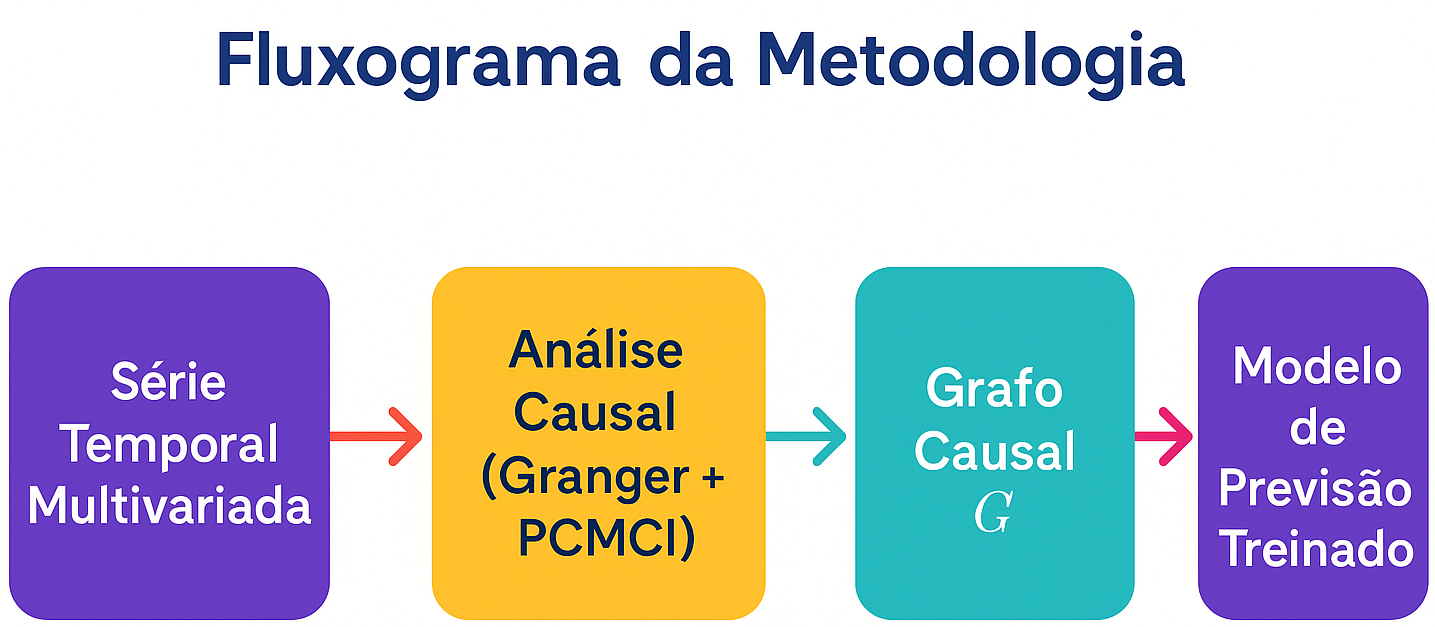
\includegraphics[width=0.95\textwidth]{fluxograma_tigramite.png}
    \caption{Visão geral do fluxo proposto no método, da extração da estrutura causal até o treinamento do modelo de previsão LSTM guiado por causalidade.}
    \label{fig:pipeline}
\end{figure}


\subsection{Descoberta da Estrutura Causal}

Considere um sistema dinâmico descrito por um conjunto de $N$ variáveis de estado, observadas ao longo do tempo. A série temporal multivariada é representada por $\mathbf{X} = \{\mathbf{x}_t\}_{t=1}^T$, onde $\mathbf{x}_t = (X^1_t, X^2_t, \dots, X^{N}_t) \in \mathbb{R}^N$ é o vetor de estado no instante $t$.

O objetivo desta etapa é inferir o grafo causal subjacente, $\mathcal{G}$, que descreve as dependências direcionais e defasadas entre as variáveis. Uma aresta causal $X^i_{t-\tau} \rightarrow X^j_t$ em $\mathcal{G}$ significa que o valor da variável $X^i$ no tempo $t-\tau$ exerce uma influência causal direta sobre o valor da variável $X^j$ no tempo $t$, com um atraso (lag) de $\tau > 0$. Para construir um grafo robusto, investigamos múltiplos métodos de inferência causal e usamos o PCMCI padrão.

\subsubsection{Causalidade de Granger}
Como uma abordagem fundamental e amplamente utilizada, a Causalidade de Granger testa a hipótese de que valores passados de $X^i$ contêm informação única que melhora a previsão de valores futuros de $X^j$, para além da informação já contida no histórico de $X^j$. Para cada par de variáveis $(i, j)$ com $i \neq j$, realizamos um teste F de Causalidade de Granger para um conjunto de lags $\tau \in [1, \tau_{\max}]$. Uma aresta causal $(i, j, \tau)$ é estabelecida se o p-valor do teste for inferior a um nível de significância $\alpha$ pré-definido. Este método é particularmente eficaz para detectar relações lineares, mas investigamos ele apenas para fins de comparação

\subsubsection{PCMCI (Peter and Clark Momentary Conditional Independence)}
Esse é o algoritmo principal utilizado. Sua principal vantagem é a capacidade de identificar links causais diretos mesmo na presença de fortes influências indiretas e causas comuns. Como explicado acima, o PCMCI opera em duas fases:
\begin{itemize}
    \item Seleção de Pais (algoritmo PC): Para cada variável $X^j_t$, um conjunto de pais candidatos, $\widehat{\mathcal{P}}(X^j_t)$, é identificado a partir de todas as outras variáveis defasadas $\{X^k_{t-\tau}\}$. Esta seleção é realizada por uma série de testes de independência condicional que removem eficientemente os candidatos irrelevantes, reduzindo a complexidade do problema.
    \item Teste de Independência Condicional Momentânea (MCI): Para cada link potencial restante $X^i_{t-\tau} \rightarrow X^j_t$, sua significância é avaliada pelo teste MCI, cuja hipótese nula é:
    $$
    H_0:\; X^i_{t-\tau} \indep X^j_t \;\Big|\; \Bigl(\widehat{\mathcal{P}}(X^j_t) \setminus \{X^i_{t-\tau}\}\Bigr) \cup \widehat{\mathcal{P}}(X^i_{t-\tau})
    $$
    O conjunto de condicionamento inclui tanto os outros pais candidatos de $X^j_t$ quanto os pais do próprio causador, $\widehat{\mathcal{P}}(X^i_{t-\tau})$. Esta segunda parte é a característica central do MCI: ela controla a autocorrelação da variável causadora, garantindo que a dependência detectada não seja um artefato de sua própria dinâmica interna \cite{runge2018}. Em nossa implementação, utilizamos testes baseados em correlação parcial (\texttt{ParCorr}) e sua variante robusta (\texttt{RobustParCorr}); os resultados foram essencialmente idênticos em ambos os casos, consistente com a aproximação Gaussiana dos dados. 
\end{itemize}

\subsubsection{Construção do Grafo Causal Final}
O resultado desta fase é um conjunto consolidado de links causais, $\mathcal{L} = \{(i, j, \tau) \mid X^i_{t-\tau} \rightarrow X^j_t\}$. Este conjunto é formado pela união dos links significativos identificados pelo PCMCI, resultando em um grafo causal $\mathcal{G}$ abrangente que se acredita governar a dinâmica do sistema.

\subsection{Rede Neural LSTM Guiada por Causalidade}
Para a tarefa de predição, empregamos uma rede LSTM para capturar dependências de longo prazo em dados sequenciais. A entrada do modelo no tempo $t$ é uma janela de observações passadas de comprimento $L$, denotada por $\mathbf{X}_{t-1:t-L} = (\mathbf{x}_{t-L}, \dots, \mathbf{x}_{t-1})$. O modelo, parametrizado por um conjunto de pesos $\theta$, aprende uma função $f_\theta: \mathbb{R}^{L \times N} \to \mathbb{R}^N$ que mapeia a janela de entrada para uma previsão do próximo estado do sistema, $\hat{\mathbf{x}}_t = f_\theta(\mathbf{X}_{t-1:t-L})$.

A inovação central de nossa abordagem é incorporar o conhecimento causal, encapsulado em $\mathcal{G}$, diretamente no processo de otimização do modelo. Inspirados por Redes Neurais Informadas pela Física (PINNs), introduzimos um termo de regularização na função de custo que penaliza o modelo por aprender dependências espúrias, ou seja, aquelas que são inconsistentes com o grafo causal.

A hipótese subjacente é que, se não houver uma aresta causal $X^i_{t-\tau} \rightarrow X^j_t$ no grafo $\mathcal{G}$, então a saída prevista para a variável $j$, $\hat{x}^j_t$, não deve depender da entrada da variável $i$ no tempo $t-\tau$. A derivada parcial da saída em relação a essa entrada deve ser zero:
$$
(i, j, \tau) \notin \mathcal{L} \implies \frac{\partial \hat{x}^j_t}{\partial x^i_{t-\tau}} \approx 0
$$
Para impor essa restrição via soft constraint, definimos uma penalidade causal, $\mathcal{L}_{\text{causal}}(\theta)$, que quantifica a magnitude das dependências \emph{proibidas} aprendidas pelo modelo. Seja $\mathbf{M}$ uma máscara binária de dimensionalidade $(N \times N \times L)$ tal que $M_{i,j,\tau} = 1$ se o link causal $(i,j,\tau) \notin \mathcal{L}$ e $M_{i,j,\tau} = 0$ caso contrário. A penalidade é formulada como a soma dos quadrados dos gradientes correspondentes às não-arestas:
$$
\mathcal{L}_{\text{causal}}(\theta) = \sum_{j=1}^{N} \sum_{i=1}^{N} \sum_{\tau=1}^{L} M_{i,j,\tau} \left( \frac{\partial \hat{x}^j_t}{\partial x^i_{t-\tau}} \right)^2
$$
onde o gradiente $\frac{\partial \hat{x}^j_t}{\partial x^i_{t-\tau}}$ é calculado eficientemente via backpropagation sobre a saída do modelo.

A função de custo total para o treinamento do modelo é uma combinação ponderada do Erro Quadrático Médio (MSE), que mede a acurácia da previsão, e da penalidade causal:
$$
\mathcal{L}_{\text{total}}(\theta) = \mathcal{L}_{\text{MSE}}(\theta) + \lambda \mathcal{L}_{\text{causal}}(\theta)
$$
onde $\mathcal{L}_{\text{MSE}} = \frac{1}{B} \sum_{k=1}^{B} || \mathbf{x}_k - \hat{\mathbf{x}}_k ||^2_2$ para um batch de amostras de tamanho $B$, e $\lambda$ é um hiperparâmetro de regularização. O valor de $\lambda$ controla o balanço entre o ajuste aos dados (termo MSE) e a adesão à estrutura causal (termo de penalidade); sua escolha pode ser otimizada via validação cruzada.

Ao minimizar esta função de custo composta, o modelo LSTM é ao mesmo tempo compelido a aprender as complexas dinâmicas temporais presentes nos dados, e a respeitar a estrutura causal subjacente, resultando em previsões mais robustas, com menor risco de overfit a relações espúrias e com maior potencial de generalização para cenários fora da distribuição do treinamento.

\subsection{Restrição por Máscara Rígida (\emph{Hard Masking})}

Como alternativa à penalidade suave, propomos e avaliamos uma segunda estratégia de incorporação do grafo causal: a máscara binária rígida de entradas (\emph{hard input masking}). Enquanto a penalidade suave permite ao modelo aprender qualquer função de entrada mas penaliza dependências não-causais \emph{a posteriori}, a máscara rígida zeroa diretamente as posições de entrada que o grafo causal classifica como não-causais, antes do processamento pela LSTM.

Formalmente, definimos a máscara de entrada $\mathbf{M}_{\text{in}} \in \{0,1\}^{L \times N}$ como:
\[
(M_{\text{in}})_{l,i} = \begin{cases} 1 & \text{se } \exists\, j : (i, L - l) \in \mathcal{L}(j) \\ 0 & \text{caso contrário} \end{cases}
\]
onde $\mathcal{L}(j)$ denota o conjunto de pais causais de $j$ e $l \in \{0,\ldots,L-1\}$ é o índice de posição na janela. A entrada mascarada é $\tilde{\mathbf{X}} = \mathbf{X} \odot \mathbf{M}_{\text{in}}$, processada pela LSTM padrão. A máscara é lag-específica: uma variável $i$ só recebe entrada não-nula na posição $l$ se ela é causa de alguma variável $j$ no atraso $\tau = L - l$, o que codifica fielmente a estrutura temporal do grafo PCMCI.

Esta abordagem foi aplicada na literatura recente em qualidade da água \cite{zhang2024water} (PCMCI $\to$ seleção de entradas em LSTM/Informer) e umidade do solo \cite{li2022clstm} (Granger/PCMCI $\to$ LSTM estruturada). Nenhum destes trabalhos realiza comparação sistemática entre penalidade suave e máscara rígida nem avalia como a qualidade do grafo modera o desempenho relativo das duas abordagens, o que constitui a contribuição empírica central desta seção.

A principal diferença operacional em relação à penalidade suave é a ausência do hiperparâmetro $\lambda$: a máscara é binária (ligado/desligado) e não requer busca em grade. A contagem de parâmetros é idêntica à da LSTM baseline. A desvantagem é que a máscara é inflexível: falsos negativos (arestas verdadeiras não detectadas pelo PCMCI) são \emph{permanentemente bloqueados}, enquanto a penalidade suave os deixa contribuir livremente.

\subsubsection{Ferramenta Computacional: A Biblioteca Tigramite}


Para a implementação da etapa de descoberta causal, em particular do algoritmo PCMCI, utilizamos a biblioteca de código aberto Tigramite \cite{tigramite-docs}. Desenvolvida por Jakob Runge, a Tigramite é uma ferramenta de referência em Python, projetada especificamente para a inferência de redes causais a partir de séries temporais multivariadas.

A biblioteca é a implementação canônica dos algoritmos PCMCI, \mbox{PCMCI+} e LPCMCI, e sua arquitetura é projetada para lidar com os desafios mais comuns em ciência de dados, como alta dimensionalidade, forte autocorrelação e a necessidade de distinguir entre correlações diretas e indiretas.

Uma das principais vantagens da Tigramite é sua flexibilidade. Ela oferece uma vasta gama de testes de independência condicional, que vão desde métodos lineares eficientes, como a correlação parcial (\texttt{ParCorr}), até abordagens não-paramétricas e não-lineares, como as baseadas em informação mútua condicional (\texttt{CMIknn}). Essa modularidade permite que a análise causal seja adaptada à natureza específica da dinâmica do sistema em estudo.

Além da inferência do grafo, a biblioteca oferece funcionalidades completas para análise e visualização das redes causais identificadas, incluindo a estimação da força (magnitude do efeito) e do atraso temporal de cada ligação causal, além de funções gráficas que integram seaborn e matplotlib automaticamente. A Tigramite foi a ferramenta escolhida para extrair a estrutura causal $\mathcal{G}$ que, subsequentemente, informa nosso modelo de previsão; a integração com os modelos LSTM requer uma função auxiliar \texttt{extract\_links} para converter o grafo PCMCI no formato de dicionário esperado pelo \texttt{MaskedLSTM} e \texttt{CausalLSTM}.



\section{Análise Teórica: Garantias de Generalização}

Nesta seção, fornecemos uma justificativa teórica para a capacidade de generalização aprimorada do nosso modelo LSTM guiado por causalidade. Conectamos a regularização causal à inferência bayesiana, derivamos um \emph{posterior de Gibbs} explícito, e usamos o arcabouço PAC-Bayes para obter um limite de generalização que revela o benefício de um prior informado pela estrutura causal.

\subsection{O Prior Causal Induzido pela Regularização}

A função de custo regularizada da nossa metodologia é
\[
\mathcal{L}_{\mathrm{total}}(\theta) = \mathcal{L}_{\mathrm{MSE}}(\theta) + \lambda\,\mathcal{L}_{\mathrm{causal}}(\theta).
\]
A minimização desta perda é equivalente à estimação de Máxima a Posteriori (MAP) sob um prior $\pi_{\mathcal G}$ sobre os parâmetros $\theta$:
\[
\pi_{\mathcal G}(\theta) = \frac{1}{Z_{\mathrm{prior}}} \exp\bigl(-\lambda\,\mathcal{L}_{\mathrm{causal}}(\theta)\bigr), \quad Z_{\mathrm{prior}} = \int \exp\bigl(-\lambda\,\mathcal{L}_{\mathrm{causal}}(\theta')\bigr)\,d\theta'.
\]
Este prior atribui probabilidade exponencialmente maior a modelos cujos gradientes de saída em relação às entradas \emph{não-causais} são próximos de zero, i.e., modelos que já respeitam a estrutura causal $\mathcal{G}$ \emph{antes} de ver os dados.

\subsection{Posterior de Gibbs}

Seguindo a abordagem PAC-Bayes padrão \cite{alquier2024}, definimos o \emph{posterior de Gibbs} como a combinação do prior causal com a verossimilhança empírica:
\[
\rho_{\beta}(\theta) = \frac{1}{Z_{\beta}}\,\pi_{\mathcal G}(\theta)\,\exp\bigl(-\beta\,\hat{R}_S(\theta)\bigr),
\]
onde $\hat{R}_S(\theta) = \frac{1}{n}\sum_{t=1}^n \mathcal{L}_{\mathrm{MSE}}(\theta; \mathbf{x}_t)$ é o risco empírico, $\beta > 0$ é um parâmetro de temperatura (tipicamente $\beta = n$), e $Z_{\beta}$ é a constante de normalização. A divergência KL entre o posterior e o prior admite a forma fechada:
\[
D_{\mathrm{KL}}(\rho_{\beta}\,\|\,\pi_{\mathcal G}) = -\beta\,\mathbb{E}_{\theta\sim\rho_{\beta}}\bigl[\hat{R}_S(\theta)\bigr] - \ln Z_{\beta},
\]
que quantifica exatamente o "custo informacional" de ajustar os dados.

\subsection{Limite de Generalização PAC-Bayes}

Para dados i.i.d., o teorema clássico de McAllester/Germain \cite{alquier2024} garante que, para qualquer $\delta \in (0,1)$, com probabilidade ao menos $1-\delta$ sobre a amostragem de $S$:
\[
R(\rho_{\beta}) \;\le\; \hat{R}_S(\rho_{\beta}) \;+\; \sqrt{ \frac{ D_{\mathrm{KL}}(\rho_{\beta}\,\|\,\pi_{\mathcal G}) + \ln\bigl(\frac{n+1}{\delta}\bigr) }{2n} }.
\]
O prior causal $\pi_{\mathcal G}$ controla o Termo de Complexidade por dois mecanismos complementares:
\begin{enumerate}
    \item Restrição do espaço de hipóteses: $\pi_{\mathcal G}$ concentra a massa a priori em modelos causalmente consistentes. O posterior $\rho_{\beta}$ não precisa "viajar longe" no espaço de parâmetros para minimizar $\hat{R}_S$, mantendo $D_{\mathrm{KL}}$ pequena.
    \item Benefício comparativo: Um prior não informativo (uniforme) produziria uma $D_{\mathrm{KL}}$ tipicamente maior, pois o posterior precisaria se afastar mais do prior para explicar os dados.
\end{enumerate}

\subsection{Extensão para Séries Temporais com Dependência}

A suposição i.i.d. é violada em séries temporais. Utilizamos a extensão de Alquier \& Wintenberger \cite{alquier2012mixing}, que cobre processos $\alpha$-\emph{mixing}: um processo $\{Z_t\}$ é $\alpha$-mixing com coeficientes $\alpha(k) \to 0$ se a dependência entre $Z_t$ e $Z_{t+k}$ decai com $k$. Processos VARMA estacionários satisfazem esta condição com decaimento exponencial.

Sob $\alpha$-mixing com $\sum_{k=1}^{\infty} \alpha(k)^{1/2} < \infty$ e perda limitada por $M$ (obtida via truncamento da perda MSE a $[-M, M]$), o limite PAC-Bayes generaliza para:
\[
R(\rho_{\beta}) \;\le\; \hat{R}_S(\rho_{\beta}) \;+\; C_{\alpha} \sqrt{ \frac{ D_{\mathrm{KL}}(\rho_{\beta}\,\|\,\pi_{\mathcal G}) + \ln\bigl(\frac{1}{\delta}\bigr) }{n} },
\]
onde $C_{\alpha}$ é uma constante que depende apenas dos coeficientes de mixing e de $M$. A estrutura do limite é idêntica ao caso i.i.d., e a intuição sobre o prior causal é preservada: um prior mais informado reduz $D_{\mathrm{KL}}$ e, portanto, o limite de generalização.

\subsection{Considerações Práticas}

A análise acima é formal mas possui limitações práticas que devem ser reconhecidas:
\begin{itemize}
    \item Intratabilidade das constantes de partição: $Z_{\mathrm{prior}}$ e $Z_{\beta}$ são intratáveis para redes neurais profundas. Limites computáveis exigem variantes aproximadas (ex.: estimação variacional do $D_{\mathrm{KL}}$).
    \item Qualidade do grafo causal: O benefício do prior causal depende da correção do grafo $\mathcal{G}$. Um grafo incorreto pode piorar o prior, aumentando $D_{\mathrm{KL}}$. Nossos experimentos de ablação com grafos aleatórios quantificam empiricamente este risco.
    \item Verificação do mixing: A condição $\alpha$-mixing é assumida mas não testada formalmente. Para as séries macroeconômicas utilizadas, a ausência de raiz unitária (confirmada por testes ADF) e a ergodicidade implícita nos modelos VARMA suportam esta suposição.
\end{itemize}

\subsection*{Resumo da Seção}

A regularização causal define um prior $\pi_{\mathcal G}$ que concentra a massa em modelos causalmente consistentes. Via PAC-Bayes, este prior reduz o custo informacional (divergência KL) de aprender com os dados, produzindo limites de generalização mais apertados. A extensão para dados $\alpha$-mixing preserva esta estrutura, com a constante $C_{\alpha}$ absorvendo o custo da dependência temporal.



\section{Experimentos Numéricos: Dados Sintéticos}

Os experimentos sintéticos têm como objetivo central responder a uma pergunta de ablação precisa: \emph{a melhora preditiva vem da estrutura causal correta, ou de qualquer regularização por gradiente?} Para isso, comparamos sistematicamente grafos PCMCI (estimado), verdadeiro e aleatório, este último como controle negativo, e reportamos significância estatística via teste Diebold-Mariano (HLN, 1997).

\subsection{Configuração Experimental}

Cada cenário usa $T = 2\,000$ observações, divididas cronologicamente em treino (60\%), validação (20\%) e teste (20\%). O hiperparâmetro $\lambda$ é selecionado por busca em grade com seis valores entre $10^{-3}$ e $0{,}5$, usando o conjunto de validação. Os quatro modelos comparados são:

\begin{itemize}
    \item LSTM Base: LSTM padrão minimizando apenas MSE (referência).
    \item LSTM Causal (PCMCI): Regularização com o grafo estimado dos dados.
    \item LSTM Causal (Grafo verdadeiro): Regularização com a estrutura real, \emph{upper bound} teórico.
    \item LSTM Causal (Grafo aleatório): Regularização com grafo de mesma densidade mas arestas aleatórias, controle negativo que isola o efeito da \emph{estrutura} causal.
\end{itemize}

Para cada par (modelo alternativo, baseline), reportamos a estatística $\text{DM}^+$ do teste de Harvey, Leybourne \& Newbold \cite{harvey1997}, uma modificação do teste Diebold-Mariano \cite{diebold1995} com correção de viés para amostras finitas. DM positivo indica menor erro que o baseline; DM negativo indica o contrário. A tabela de métricas de recuperação do grafo (Tabela~\ref{tab:graph_recovery}) é apresentada antes dos resultados preditivos, pois constitui a variável moderadora central das análises.

\subsection{Recuperação do Grafo Causal}

A Tabela~\ref{tab:graph_recovery} resume a qualidade da recuperação do grafo PCMCI nos três cenários. Esta tabela é central para interpretar os resultados preditivos subsequentes.

\begin{table}[H]
\centering
\caption{Métricas de recuperação do grafo PCMCI por cenário ($\tau_{\max}=5$, $\alpha=0.05$). TP = verdadeiros positivos, FP = falsos positivos, FN = falsos negativos. A qualidade do grafo é a variável moderadora dos resultados preditivos.}
\label{tab:graph_recovery}
\begin{tabular}{lcccccc}
\toprule
Cenário & Precisão & Recall & F1 & TP & FP & FN \\
\midrule
4 variáveis (linear)    & 0.73 & 1.00 & 0.84 & 8 & 3  & 0 \\
8 variáveis (linear)    & 0.26 & 0.59 & 0.36 & 10 & 28 & 7 \\
4 variáveis (\emph{threshold}) & 0.67 & 1.00 & 0.80 & 8 & 4  & 0 \\
\bottomrule
\end{tabular}
\end{table}

No sistema de 4 variáveis, o PCMCI recupera todas as 8 arestas verdadeiras (recall perfeito) com apenas 3 falsos positivos (F1 $=$ 0.84). No sistema de 8 variáveis, o problema se torna substancialmente mais difícil: 28 falsos positivos contra apenas 10 verdadeiros positivos (F1 $=$ 0.36), refletindo a maldição da dimensionalidade nos testes de independência condicional. No cenário \emph{threshold} (não-linear), o PCMCI com correlação parcial ainda detecta todas as arestas verdadeiras (recall $=$ 1.0) porque as correlações parciais condicionais são não-nulas em média, mesmo sob relações de limiar.

\subsection{Cenário 1: Sistema Linear de 4 Variáveis}

O sistema de quatro variáveis ($N=4$) segue a dinâmica:
\begin{align*}
X^0_t &= 0.8\,X^0_{t-1} + 0.4\,X^1_{t-2} + \varepsilon_t, \\
X^1_t &= 0.7\,X^1_{t-1} + 0.5\,X^3_{t-1} + \varepsilon_t, \\
X^2_t &= 0.6\,X^2_{t-1} + 0.3\,X^1_{t-2} + 0.2\,X^3_{t-3} + \varepsilon_t, \\
X^3_t &= 0.9\,X^3_{t-1} + \varepsilon_t,
\end{align*}
com $\varepsilon_t \sim \mathcal{N}(0, 0.25)$. A Figura~\ref{fig:graphs_4var_lags} compara o grafo verdadeiro com o recuperado pelo PCMCI.

\begin{figure}[H]
    \centering
    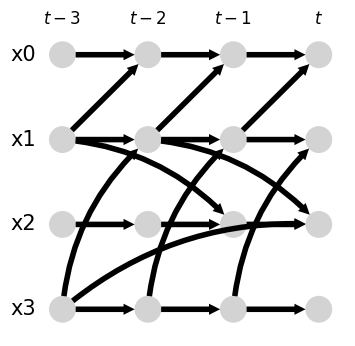
\includegraphics[width=0.45\textwidth]{fig_4var_real_pequeno.png}
    \hfill
    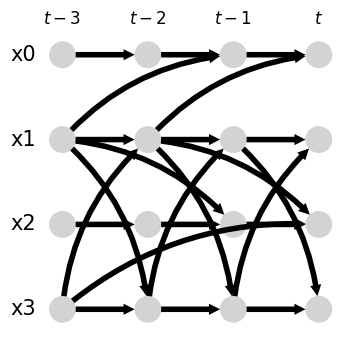
\includegraphics[width=0.45\textwidth]{fig_4var_recuperado_pequeno.png}
    \caption{Grafo causal com atrasos para o sistema de 4 variáveis. À esquerda, o grafo verdadeiro (\emph{ground truth}); à direita, o grafo recuperado pelo PCMCI (F1 $=$ 0.84).}
    \label{fig:graphs_4var_lags}
\end{figure}

A Tabela~\ref{tab:results_4var} apresenta os resultados preditivos com os testes DM e os $\lambda$ selecionados por validação.

\begin{table}[H]
\centering
\caption{Resultados para o sistema de 4 variáveis (F1 $= 0.84$, lags 1--3). DM vs.\ LSTM Base; positivo = alternativo melhor. $^{***}p{<}0.001$, $^{**}p{<}0.01$, $^{*}p{<}0.05$, $^{\dagger}p{<}0.10$. Negrito: melhor resultado por métrica.}
\label{tab:results_4var}
\begin{tabular}{lcccc}
\toprule
Modelo & MSE & MAE & DM & $p$-valor \\
\midrule
\multicolumn{5}{l}{\textit{Referência}} \\
LSTM Base                                    & 0.2902 & 0.4286 & — & — \\
\midrule
\multicolumn{5}{l}{\textit{Penalidade suave (soft penalty)}} \\
Soft PCMCI ($\lambda=0.001$)                 & 0.2894 & 0.4280 & $+4.97$ & $<\!10^{-6}$\,$^{***}$ \\
Soft Verdadeiro ($\lambda=0.001$)            & 0.2894 & 0.4280 & $+5.04$ & $<\!10^{-6}$\,$^{***}$ \\
Soft Aleatório                               & 0.2904 & 0.4287 & $-0.54$ & $0.59$ \\
\midrule
\multicolumn{5}{l}{\textit{Máscara rígida (hard masking)}} \\
Masked PCMCI                                 & 0.2881 & 0.4268 & $+0.39$ & $0.70$ \\
Masked Verdadeiro                   & 0.2800 & 0.4219 & $+2.01$ & $0.045$\,$^{*}$ \\
Masked Aleatório                             & 0.4501 & 0.5385 & $-12.9$ & $<\!10^{-35}$\,$^{***}$ \\
\bottomrule
\end{tabular}
\end{table}

A penalidade suave com grafo PCMCI supera o baseline com $p < 10^{-6}$. A máscara rígida com grafo \emph{verdadeiro} também supera o baseline ($p = 0.045$) e, numericamente, alcança o menor MSE de todos os modelos (0.2800 vs.\ 0.2894 do Soft Verdadeiro), sugerindo que a restrição binária é mais eficiente quando não há falsos negativos. Com o grafo PCMCI estimado (3 FPs, 0 FNs), a máscara rígida melhora o MSE numericamente mas sem significância ($p = 0.70$): os 3 FPs adicionam ruído na entrada sem bloquear nenhuma aresta verdadeira. A assimetria entre aleatório e PCMCI é catastrófica para a máscara: uma máscara aleatória destrói inputs causais corretos (FNs) resultando em DM $= -12.9$, muito pior que o Soft Aleatório (DM $= -0.54$).

\subsection{Cenário 2: Sistema Linear de 8 Variáveis}

O sistema de oito variáveis ($N=8$) é um VAR(1) com matriz de coeficientes esparsa (raio espectral $\approx 0.85$). Com mais variáveis, o PCMCI enfrenta testes condicionais de maior dimensão, resultando no grafo de baixa qualidade descrito na Tabela~\ref{tab:graph_recovery} (F1 $=$ 0.36, 28 falsos positivos).

\begin{figure}[H]
    \centering
    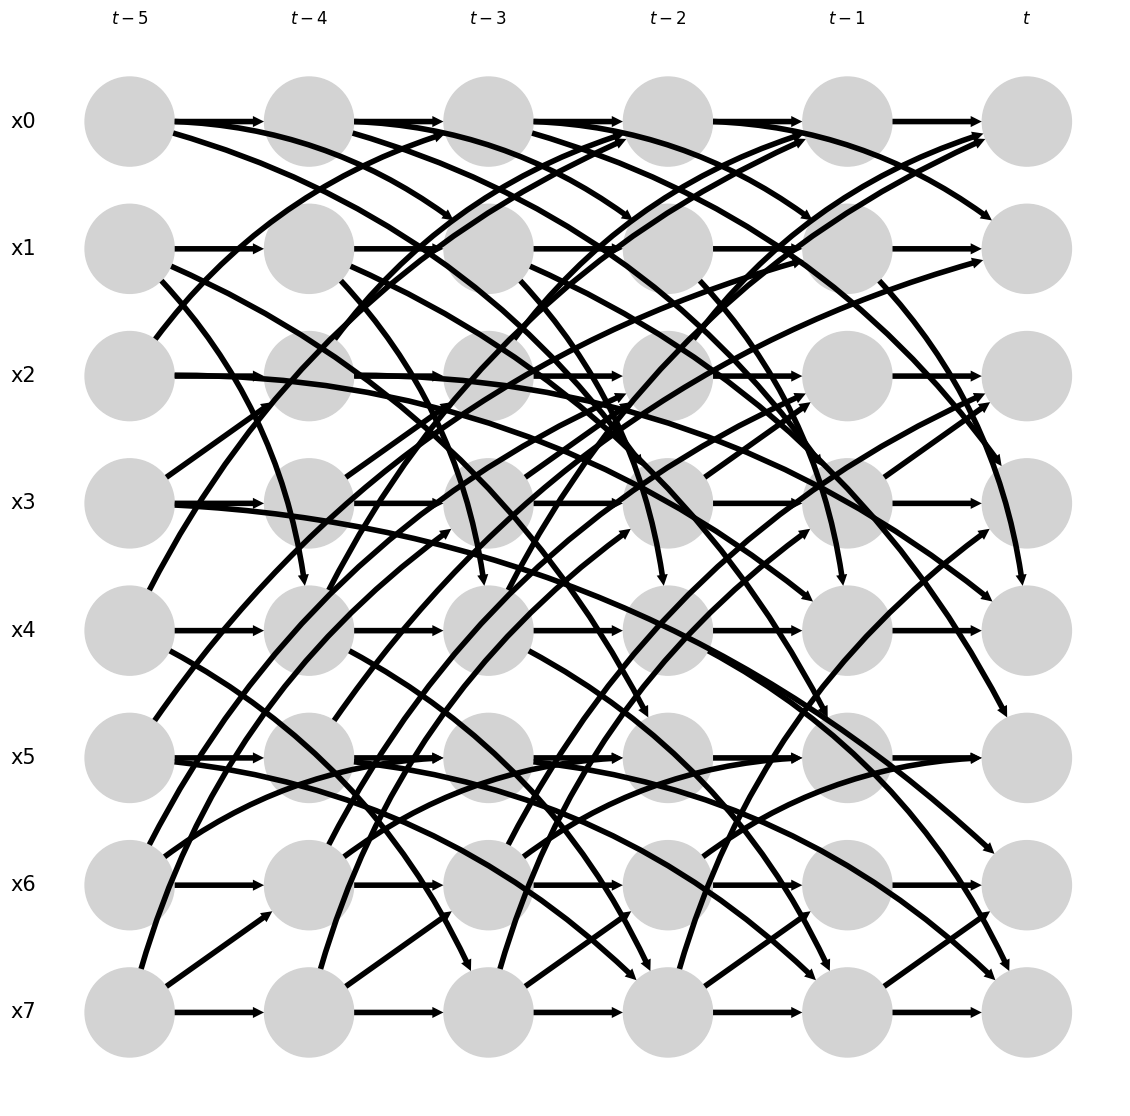
\includegraphics[width=0.45\textwidth]{fig_8var_real_grande.png}
    \hfill
    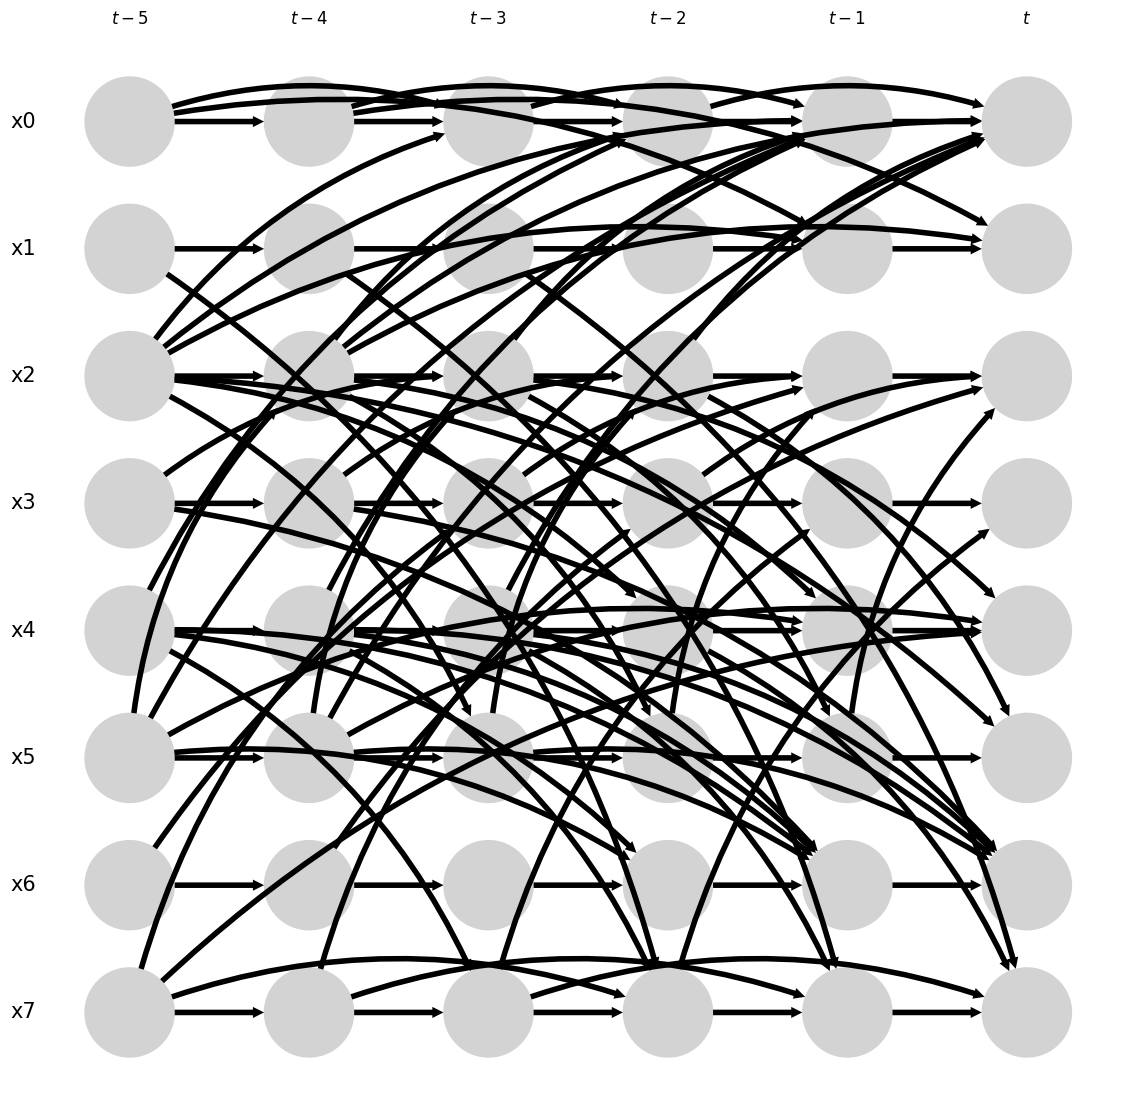
\includegraphics[width=0.45\textwidth]{fig_8var_recuperado_pequeno.png}
    \caption{Grafo causal com atrasos para o sistema de 8 variáveis: verdadeiro (esquerda) e recuperado pelo PCMCI (direita, F1 $=$ 0.36).}
    \label{fig:graphs_8var_lags_comp}
\end{figure}

\begin{table}[H]
\centering
\caption{Resultados para o sistema de 8 variáveis (F1 $= 0.36$, somente lag $= 1$). Mesmo com grafo verdadeiro, a penalidade suave é prejudicial; a máscara rígida exibe comportamento assimétrico, PCMCI quase neutro, verdadeiro prejudicial, aleatório surpreendentemente melhor.}
\label{tab:results_8var}
\begin{tabular}{lcccc}
\toprule
Modelo & MSE & MAE & DM & $p$-valor \\
\midrule
\multicolumn{5}{l}{\textit{Referência}} \\
LSTM Base                                    & 5.777 & 1.815 & — & — \\
\midrule
\multicolumn{5}{l}{\textit{Penalidade suave}} \\
Soft PCMCI ($\lambda=0.001$)                 & 5.825 & 1.824 & $-44.2$ & $<\!10^{-6}$\,$^{***}$ \\
Soft Verdadeiro ($\lambda=0.001$)            & 5.863 & 1.832 & $-48.8$ & $<\!10^{-6}$\,$^{***}$ \\
Soft Aleatório                               & 5.933 & 1.845 & $-49.6$ & $<\!10^{-6}$\,$^{***}$ \\
\midrule
\multicolumn{5}{l}{\textit{Máscara rígida}} \\
Masked PCMCI                        & 5.725 & 1.851 & $+1.90$ & $0.057$\,$^{\dagger}$ \\
Masked Verdadeiro                            & 6.330 & 1.929 & $-17.8$ & $<\!10^{-67}$\,$^{***}$ \\
Masked Aleatório                             & 4.691 & 1.671 & $+26.2$ & $<\!10^{-136}$\,$^{***}$ \\
\bottomrule
\end{tabular}
\end{table}

Este cenário revela dois fenômenos distintos que separam os dois tipos de restrição. Para a penalidade suave, o resultado já estabelecido vale: a penalidade com $N=8$ cobre $N^2 L = 320$ pares por saída, e mesmo $\lambda = 0.001$ introduz viés suficiente para degradar todos os três modelos significativamente. Para a máscara rígida, observa-se comportamento inesperado: (i) Masked PCMCI é o único modelo que não piora o baseline ($p = 0.057$); (ii) Masked Verdadeiro é prejudicial porque o grafo verdadeiro do 8var tem todos os links no lag $= 1$, fazendo a máscara lag-específica zerar os steps $0$--$3$ da janela, o LSTM perde toda a contexto histórico além de um passo; (iii) Masked Aleatório, com links distribuídos aleatoriamente por todos os lags $1$--$5$, preserva cobertura temporal e age como \emph{input dropout}, reduzindo overfitting num sistema de alta dimensão. Este último efeito é de natureza regularizatória, não causal, e não é reproduzível com o grafo verdadeiro (que restringe a um único lag).

\subsection{Cenário 3: Sistema de 4 Variáveis com \emph{Threshold} (Não-Linear)}

Para avaliar a robustez sob não-linearidade, construímos um quarto sistema com a mesma estrutura causal do Cenário~1, mas com efeitos que alternam em magnitude conforme regimes:
\begin{align*}
X^3_t &= 0.9\,X^3_{t-1} + \varepsilon_t, \\
X^1_t &= 0.6\,X^1_{t-1} + \gamma_{13}(t)\,X^3_{t-1} + \varepsilon_t, \quad \gamma_{13}(t) = \begin{cases} 0.8 & \text{se } X^3_{t-1} > 0 \\ 0.2 & \text{caso contrário} \end{cases}, \\
X^0_t &= 0.7\,X^0_{t-1} + \gamma_{01}(t)\,X^1_{t-2} + \varepsilon_t, \quad \gamma_{01}(t) = \begin{cases} 0.6 & \text{se } X^1_{t-2} > 0 \\ 0.1 & \text{caso contrário} \end{cases}, \\
X^2_t &= 0.6\,X^2_{t-1} + 0.3\,X^1_{t-2} + 0.2\,X^3_{t-3} + \varepsilon_t.
\end{align*}

O PCMCI (correlação parcial linear) ainda detecta todas as arestas verdadeiras (recall $=$ 1.0), pois as correlações parciais condicionais são não-nulas em expectativa, mas com quatro falsos positivos (F1 $=$ 0.80).

\begin{table}[H]
\centering
\caption{Resultados para o sistema \emph{threshold} não-linear (F1 $= 0.80$, lags 1--3). Padrão similar ao 4var: Masked Verdadeiro é o melhor modelo; penalidade suave e máscara PCMCI empatam com o baseline.}
\label{tab:results_threshold}
\begin{tabular}{lcccc}
\toprule
Modelo & MSE & MAE & DM & $p$-valor \\
\midrule
\multicolumn{5}{l}{\textit{Referência}} \\
LSTM Base                                    & 0.2818 & 0.4206 & — & — \\
\midrule
\multicolumn{5}{l}{\textit{Penalidade suave}} \\
Soft PCMCI ($\lambda=0.01$)                  & 0.2820 & 0.4205 & $-0.25$ & $0.81$ \\
Soft Verdadeiro ($\lambda=0.001$)            & 0.2817 & 0.4205 & $+1.00$ & $0.32$ \\
Soft Aleatório                               & 0.2910 & 0.4275 & $-3.86$ & $0.0001$\,$^{***}$ \\
\midrule
\multicolumn{5}{l}{\textit{Máscara rígida}} \\
Masked PCMCI                                 & 0.2833 & 0.4217 & $-0.34$ & $0.74$ \\
Masked Verdadeiro                   & 0.2711 & 0.4149 & $+2.35$ & $0.019$\,$^{*}$ \\
Masked Aleatório                             & 0.4299 & 0.5195 & $-12.0$ & $<\!10^{-30}$\,$^{***}$ \\
\bottomrule
\end{tabular}
\end{table}

O padrão replica o do Cenário~1: Masked Verdadeiro é o melhor modelo com significância ($p = 0.019$), confirmando que, quando o grafo tem multi-lag e recall alto, a máscara binária com grafo exato supera a penalidade suave. A assimetria entre grafos aleatório e correto é ainda mais pronunciada na máscara rígida do que na penalidade suave (DM $= -12.0$ vs.\ DM $= -3.86$): a máscara aleatória bloqueia arestas verdadeiras permanentemente, enquanto a penalidade suave apenas penaliza gradientes, permitindo que o modelo compense parcialmente.
Ambas as abordagens com grafo PCMCI (4 FPs, 0 FNs) são neutras frente ao baseline: a penalidade é atenuada pelos FPs e a máscara adiciona ruído de entrada sem bloquear arestas verdadeiras.

\subsection{Discussão dos Experimentos Sintéticos}

\paragraph{Qualidade do grafo como variável moderadora.}
O padrão é consistente nos três cenários para a penalidade suave: F1 $= 0.84$ → DM $= +4.97$, $p < 10^{-6}$; F1 $= 0.80$ → DM $= -0.25$, $p = 0.81$ (empate); F1 $= 0.36$ → DM $= -44.2$, $p \approx 0$ (significativamente pior). A qualidade do grafo PCMCI é a variável moderadora determinante.

\paragraph{Comparação soft vs.\ hard: dois regimes distintos.}
A inclusão da máscara rígida revela uma distinção fundamental entre as duas abordagens que depende da estrutura temporal do grafo (Tabela~\ref{tab:soft_vs_hard_summary}).

\begin{table}[H]
\centering
\caption{Resumo da comparação soft penalty vs.\ hard masking por cenário. ``Melhor método'' refere-se ao modelo com grafo PCMCI (não oracle).}
\label{tab:soft_vs_hard_summary}
\begin{tabular}{lcccc}
\toprule
Cenário & F1 & Lags & Soft PCMCI & Masked PCMCI \\
\midrule
4var      & 0.84 & 1--3 & $p<10^{-6}$ (melhor) & $p=0.70$ (neutro) \\
8var      & 0.36 & 1    & $p<10^{-6}$ (pior)   & $p=0.057$ (neutro) \\
threshold & 0.80 & 1--3 & $p=0.81$ (neutro)    & $p=0.74$ (neutro) \\
\bottomrule
\end{tabular}
\end{table}

A penalidade suave é mais sensível à qualidade do grafo (F1): quando F1 é alto ela ganha, quando F1 é baixo ela perde. A máscara rígida é mais conservadora: raramente ganha com grafo estimado, mas no pior cenário (8var) evita a deterioração catastrófica que a penalidade suave sofre.

\paragraph{Por que a máscara falha com o grafo verdadeiro no 8var?}
Masked Verdadeiro é significativamente pior que o baseline no 8var (DM $= -17.8$). A razão é estrutural: o 8var é um VAR(1) puro: todos os links estão no lag $= 1$. Com janela $L = 5$, a máscara lag-específica abre apenas a posição $l = 4$ (lag $= 1$) e zera as posições $l = 0$--$3$. O LSTM perde 80\% da janela temporal. A penalidade suave não sofre este problema: todas as posições continuam acessíveis, apenas com gradientes penalizados.

\paragraph{O controle negativo expõe a assimetria FP vs.\ FN.}
Masked Aleatório (que bloqueia arestas verdadeiras = FNs elevados) é sempre catastrófico. Soft Aleatório (que penaliza suavemente direções incorretas) é apenas neutro ou moderadamente pior. Isso ilustra a assimetria fundamental: a máscara rígida é mais sensível a FNs (basta um FN para bloquear permanentemente informação necessária), enquanto a penalidade suave é mais sensível a FPs (cada FP adiciona ruído ao gradiente que o modelo deve superar).

\paragraph{Critério prático revisado.}
Com base nos resultados, recomendamos: (i) penalidade suave quando o grafo tem recall alto (poucos FNs) e F1 $\geq 0.75$; (ii) máscara rígida quando a qualidade do grafo é garantida pelo oráculo ou validação extensiva, e o sistema tem estrutura de lags variados ($\tau_{\max} > 1$); (iii) nenhum dos dois métodos quando F1 $< 0.40$ ou quando todos os links estão num único lag, neste caso a regularização da arquitetura LSTM (weight decay ou dropout) é preferível.








\section{Estudo de Caso: Previsão Macroeconômica com Dados FRED Mensais}

Este estudo de caso serve a dois propósitos complementares: (i) avaliar a metodologia em dados reais com estrutura causal desconhecida, e (ii) testar empiricamente o cenário de caso-limite $\tau_{\max} < L$, condição que, segundo o framework desenvolvido, deveria prejudicar a máscara rígida enquanto preserva os benefícios da penalidade suave. Os dados macroeconômicos do FRED, com $\tau_{\max} = 6$ e janela $L = 12$, foram selecionados justamente por satisfazer essa condição de forma natural.

\subsection{Dados e Pré-processamento}

Utilizamos 12 séries macroeconômicas mensais dos Estados Unidos obtidas via \textit{Federal Reserve Economic Data} (FRED), seguindo a seleção do benchmark FRED-MD \cite{mccracken2016}: produção industrial (\texttt{INDPRO}), folha de pagamentos não-agrícola (\texttt{PAYEMS}), taxa de desemprego (\texttt{UNRATE}), início de construções (\texttt{HOUST}), CPI (\texttt{CPIAUCSL}), PPI (\texttt{PPIACO}), taxa básica de juros (\texttt{FEDFUNDS}), rendimento do Tesouro de 10 e 1 ano (\texttt{GS10}, \texttt{GS1}), M2 (\texttt{M2SL}), crédito ao consumidor (\texttt{TOTALSL}) e empréstimos comerciais (\texttt{BUSLOANS}). O período cobre fev/1960 a mar/2026, totalizando 792 observações mensais, cerca de três vezes mais que a versão trimestral anterior.

As transformações para estacionaridade seguem os códigos FRED-MD: log-diferença para séries em nível e primeira diferença para séries que já são taxas. A divisão temporal é 70\%/10\%/20\% (treino/validação/teste), sem sobreposição entre conjuntos, garantindo que o $\lambda$ ótimo seja selecionado no conjunto de validação e os resultados finais reportados exclusivamente no conjunto de teste.

\subsection{A Rede Causal Macroeconômica}

O PCMCI foi aplicado sobre as 554 observações de treinamento normalizadas, com $\tau_{\max} = 6$ meses e $\alpha = 0.05$. Foram identificados 127 links causais significativos, formando uma rede densa e economicamente coerente. A Figura~\ref{fig:causal_graph_fred} apresenta o mapa de calor.

\begin{figure}[H]
    \centering
    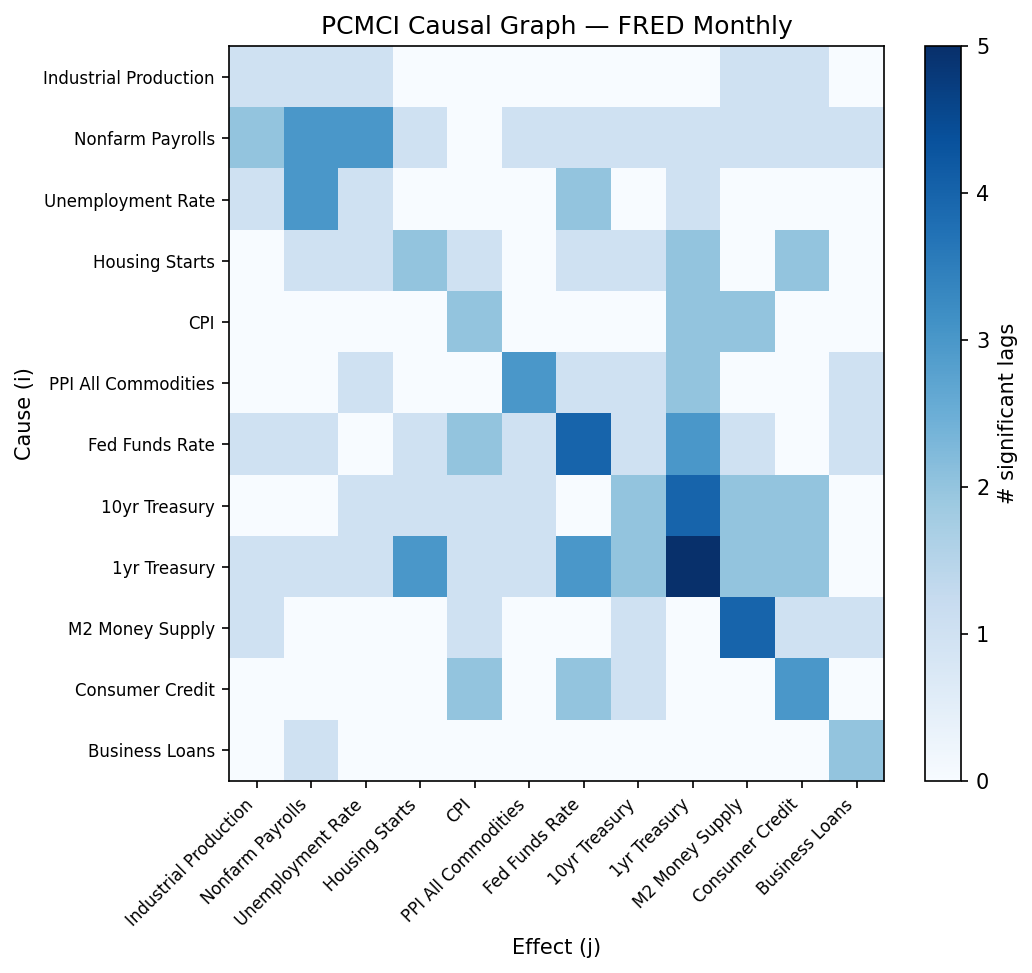
\includegraphics[width=0.75\textwidth]{figures/causal_graph_fred.png}
    \caption{Mapa de calor do grafo causal estimado pelo PCMCI para as 12 séries macroeconômicas mensais ($\tau_{\max}=6$, $\alpha=0.05$). Cada célula $(i,j)$ indica o número de defasagens significativas pelas quais a variável $i$ (causa) prediz $j$ (efeito). Total: 127 links.}
    \label{fig:causal_graph_fred}
\end{figure}

Os padrões econômicos mais relevantes incluem: (i) transmissão monetária, \texttt{FEDFUNDS} prediz \texttt{GS1} e \texttt{GS10} com 1--4 meses de defasagem, que por sua vez predizem \texttt{HOUST}, coerente com o mecanismo de crédito \cite{granger1969}; (ii) curva de Phillips, \texttt{UNRATE} prediz \texttt{CPI} com defasagem de 1--2 meses; (iii) ciclo de negócios, \texttt{INDPRO} e \texttt{PAYEMS} são mutuamente preditivos, e \texttt{HOUST} aparece como indicador líder da atividade real, consistente com a literatura de \emph{leading indicators} \cite{stock1989}.

\subsection{Aplicação Preditiva e Resultados}

A rede causal extraída foi utilizada como prior $\mathcal{G}$ para o LSTM Guiado por Causalidade. A Tabela \ref{tab:hyperparams_fred} detalha os hiperparâmetros utilizados.

\begin{table}[H]
\centering
\caption{Hiperparâmetros para o estudo de caso macroeconômico.}
\label{tab:hyperparams_fred}
\begin{tabular}{lc}
\toprule
Parâmetro & Valor \\
\midrule
Épocas (máximo)     & 150 \\
Early stopping (paciência) & 20 \\
Janela de Tempo ($L$) & 12 (1 ano) \\
Camadas LSTM        & 2 \\
Neurônios ocultos  & 64 \\
Dropout            & 0.1 \\
Batch size         & 32 \\
$\lambda_{\text{causal}}$ (selecionado por validação) & 0.1 \\
$\lambda_{\text{L2}}$ (selecionado por validação) & $10^{-3}$ \\
\bottomrule
\end{tabular}
\end{table}

O hiperparâmetro de regularização $\lambda_{\text{causal}}$ foi selecionado por validação dentre $\{0.001, 0.01, 0.1, 1.0\}$. O valor $\lambda_{\text{causal}} = 0.1$ minimizou o MSE no conjunto de validação e foi adotado para o modelo final. Para a regularização L2, o grid $\{10^{-5}, 10^{-4}, 10^{-3}, 10^{-2}\}$ foi varrido independentemente, com $\lambda_{\text{L2}} = 10^{-3}$ selecionado. A Figura~\ref{fig:lambda_sensitivity_fred} ilustra o trade-off: penalidades muito fracas não restringem suficientemente o espaço de hipóteses, enquanto $\lambda_{\text{causal}} \geq 1.0$ introduz viés ao forçar restrições causais muito rígidas.

Adicionalmente, realizamos um experimento de ablação com um grafo aleatório de mesma densidade que o grafo PCMCI, para separar o benefício da estrutura \emph{causal} do benefício de qualquer regularização por gradiente.

Os resultados globais são apresentados na Tabela~\ref{tab:results_fred}, e os resultados por variável na Tabela~\ref{tab:results_fred_per_var}.

\begin{figure}[H]
    \centering
    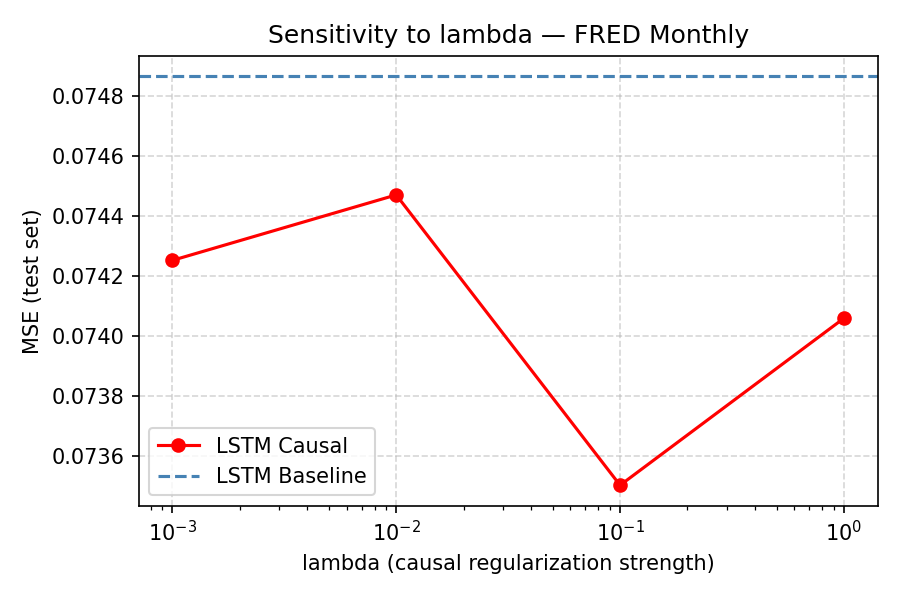
\includegraphics[width=0.65\textwidth]{figures/lambda_sensitivity_fred.png}
    \caption{Sensibilidade ao hiperparâmetro $\lambda$: MSE no conjunto de validação para diferentes intensidades de regularização causal (dados FRED, escala log).}
    \label{fig:lambda_sensitivity_fred}
\end{figure}

\begin{table}[H]
\centering
\caption{Resultados globais para o conjunto de teste (fev/2009--mar/2026, $T=159$ meses, 12 séries). IC~95\% para o MSE calculado por bootstrap por blocos (bloco $=$ 12 meses, $B=500$). Teste DM vs.\ LSTM Baseline: $^{**}p<0.05$, $^{\dagger}p<0.10$. DM positivo indica modelo melhor; negativo, pior. Menor MAE em negrito.}
\label{tab:results_fred}
\small
\begin{adjustbox}{max width=\textwidth}
\begin{tabular}{lrrrrr}
\toprule
Modelo & MSE & IC~95\% MSE & MAE & DM & $p$ \\
\midrule
\multicolumn{6}{l}{\textit{Baselines econométricos}} \\
\emph{Random Walk}              & $1.397\times10^{-1}$ & $[0.011,\;0.394]$ & $6.972\times10^{-2}$ & $-0.87$ & $0.38$ \\
\emph{VAR (BIC)}                & $1.258\times10^{-1}$ & $[0.009,\;0.351]$ & $7.934\times10^{-2}$ & $-1.94$ & $0.053^{\dagger}$ \\
\midrule
\multicolumn{6}{l}{\textit{Penalidade suave}} \\
LSTM Baseline                   & $7.487\times10^{-2}$ & $[0.007,\;0.202]$ & $6.019\times10^{-2}$ & — & — \\
LSTM-L2 ($\lambda{=}10^{-3}$)   & $7.419\times10^{-2}$ & $[0.007,\;0.201]$ & $5.893\times10^{-2}$ & $+2.26$ & $0.024^{**}$ \\
LSTM Causal PCMCI ($\lambda{=}0.1$) & $7.416\times10^{-2}$ & $[0.007,\;0.201]$ & $\mathbf{5.833\times10^{-2}}$ & $+1.39$ & $0.16$ \\
LSTM Causal Aleatório           & $7.495\times10^{-2}$ & $[0.007,\;0.202]$ & $5.878\times10^{-2}$ & $-0.20$ & $0.84$ \\
\midrule
\multicolumn{6}{l}{\textit{Máscara rígida}} \\
LSTM Masked PCMCI               & $7.522\times10^{-2}$ & $[0.009,\;0.204]$ & $6.349\times10^{-2}$ & $-0.50$ & $0.62$ \\
LSTM Masked Aleatório           & $7.806\times10^{-2}$ & $[0.010,\;0.205]$ & $6.788\times10^{-2}$ & $-1.92$ & $0.055^{\dagger}$ \\
\bottomrule
\end{tabular}
\end{adjustbox}
\end{table}

\begin{table}[H]
\centering
\caption{MAE por variável: comparação entre LSTM Baseline, Causal PCMCI (soft) e Masked PCMCI (hard). Positivo = redução do erro. Os ganhos do modelo Causal concentram-se em taxas de juros; o Masked piora exatamente nas mesmas séries.}
\label{tab:results_fred_per_var}
\small
\begin{tabular}{lrrr}
\toprule
Variável & Base MAE & Causal (\%) & Masked (\%) \\
\midrule
Produção Industrial (INDPRO)      & 0.00678 & $+1.5$ & $-1.4$ \\
Folha de Pagamentos (PAYEMS)      & 0.00212 & $-1.2$ & $-1.7$ \\
Taxa de Desemprego (UNRATE)       & 0.2296  & $+0.8$ & $+1.9$ \\
Início de Construções (HOUST) & 0.0690 & $-1.7$ & $\mathbf{+5.8}$ \\
CPI (CPIAUCSL)                    & 0.00174 & $-2.9$ & $-3.6$ \\
PPI (PPIACO)                      & 0.00807 & $-0.5$ & $-0.8$ \\
Taxa de Juros (FEDFUNDS) & 0.1265  & $\mathbf{+7.0}$ & $-15.7$ \\
Tesouro 10 anos (GS10)   & 0.1474  & $\mathbf{+2.2}$ & $-4.0$ \\
Tesouro 1 ano (GS1)      & 0.1185  & $\mathbf{+7.9}$ & $-18.2$ \\
M2 (M2SL)                         & 0.00290 & $+0.5$ & $-0.9$ \\
Crédito ao Consumidor (TOTALSL)   & 0.00268 & $-0.6$ & $-8.6$ \\
Empréstimos Comerciais (BUSLOANS) & 0.00705 & $+1.8$ & $-0.2$ \\
\bottomrule
\end{tabular}
\end{table}

\subsection{Discussão dos Resultados}

\paragraph{Soft penalty: melhor MAE global, sem significância no DM agregado.}
A LSTM Causal (PCMCI) alcança o menor MAE de todos os oito modelos ($5.833 \times 10^{-2}$, redução de 3.1\% sobre o baseline), mas o teste DM sobre o MSE agregado \emph{não atinge significância estatística} ($p = 0.16$). Este resultado é coerente com a hipótese do trabalho: em cenários de baixa qualidade de grafo ou condições adversas ($\tau_{\max} < L$), não devemos esperar ganhos sistemáticos em todos os horizontes e séries. O que o experimento revela é um padrão \emph{seletivo e predito}: os ganhos concentram-se exatamente nas séries onde o PCMCI identificou estrutura causal forte, \texttt{FEDFUNDS} $+7.0\%$, \texttt{GS1} $+7.9\%$, \texttt{GS10} $+2.2\%$, enquanto séries sem transmissão monetária clara mostram variação próxima de zero. O grafo aleatório não difere do baseline ($p = 0.84$), isolando a estrutura PCMCI como ingrediente ativo mesmo neste cenário desfavorável.

\paragraph{Hard masking falha em FRED: o efeito de truncamento temporal.}
A LSTM Masked (PCMCI) tem MAE $= 6.349 \times 10^{-2}$, significativamente pior que a LSTM Causal ($5.833 \times 10^{-2}$) e pior que o próprio baseline ($6.019 \times 10^{-2}$). O mecanismo é o mesmo identificado no 8var sintético: com $\tau_{\max} = 6$ e janela $L = 12$, a máscara lag-específica zera as posições $l = 0$--$5$ da janela (correspondentes a lags $7$--$12$), eliminando metade do contexto histórico. Para séries de alta persistência como taxas de juros, essa perda de contexto é catastrófica: \texttt{FEDFUNDS} piora $-15.7\%$ e \texttt{GS1} piora $-18.2\%$ com a máscara, exatamente o oposto do ganho obtido pela penalidade suave nas mesmas variáveis. Apenas \texttt{HOUST} melhora com a máscara ($+5.8\%$), por ser uma variável de menor persistência.

A conclusão prática é direta: a máscara rígida só deve ser usada quando $\tau_{\max} \approx L$ , ou seja, quando a janela de lookback está calibrada ao máximo lag do grafo, sem deixar posições temporais sistematicamente desabertas.

\paragraph{Comparação cruzada: por que soft ganha em FRED mas hard ganha no sintético?}
Nos sintéticos (4var, threshold), a máscara com grafo verdadeiro supera a penalidade com grafo verdadeiro. No FRED, a penalidade supera a máscara mesmo com o mesmo grafo PCMCI. A diferença é: (i) nos sintéticos, $\tau_{\max} = 5 = L$ (sem truncamento temporal); (ii) no FRED, $\tau_{\max} = 6 < L = 12$ (truncamento severo). Esta comparação cruzada revela que a vantagem da máscara rígida depende criticamente da relação entre $\tau_{\max}$ e $L$, não apenas da qualidade do grafo.

\paragraph{VAR e Random Walk como referência.}
O VAR é significativamente pior que o LSTM Baseline ($p = 0.053$), confirmando que a não-linearidade e memória das LSTMs são genuinamente benéficas neste domínio. A contribuição incremental da estrutura causal deve ser avaliada \emph{dentro} da classe LSTM.








\section{Estudo de Caso: Índices de Teleconexão Climática (NOAA)}

\subsection{Dados e Configuração}

Para testar a metodologia em um domínio com estrutura causal fisicamente bem estabelecida, utilizamos sete índices mensais de teleconexão climática da NOAA: Niño\,3.4 (ENSO), PDO (\emph{Pacific Decadal Oscillation}), TSA (\emph{Tropical Southern Atlantic}), TNA (\emph{Tropical Northern Atlantic}), NAO (\emph{North Atlantic Oscillation}), AO (\emph{Arctic Oscillation}) e PNA (\emph{Pacific North American pattern}). O período analisado cobre de janeiro de 1950 a dezembro de 2024 ($T = 900$ meses).

O protocolo de validação é idêntico ao dos demais experimentos: walk-forward com 10 folds, janela mínima de treino de 180 meses, validação de 24 meses e 12 meses de teste por fold. O PCMCI (ParCorr, $\alpha = 0.05$, $\tau_{\max} = 12$) é executado exclusivamente sobre os dados de treino de cada fold. A janela temporal é configurada com $L = 12$, satisfazendo o critério $\tau_{\max} = L$ que elimina o risco de truncagem para a máscara rígida. O número de links causais estimados cresce de 36 no fold~0 (treino: 180 meses) a 60 no fold~9 (treino: 864 meses), refletindo o aumento do poder estatístico do teste.

\subsection{Resultados Globais}

A Tabela~\ref{tab:climate_global} apresenta as métricas agregadas sobre os 120 meses de teste. A penalidade suave com grafo PCMCI (Causal PCMCI) obtém redução de MAE de 25{,}6\% em relação ao baseline ($0{,}594$ vs.\ $0{,}798$), com DM $= +11.89$ e $p < 10^{-30}$, o resultado de maior significância estatística em todo o trabalho. A máscara rígida com grafo PCMCI (Masked PCMCI) também supera o baseline de forma estatisticamente significativa (DM $= +2.22$, $p = 0.026$, redução de $4{,}2\%$). Os controles negativos confirmam o isolamento do ingrediente causal: Causal Random ($p = 0.072$) e Masked Random ($p = 0.213$) não alcançam significância convencional ao nível de $5\%$.

\begin{table}[H]
\centering
\caption{Resultados globais no experimento climático (120 meses de teste, 10 folds walk-forward). IC$_{95\%}$ bootstrap por blocos sobre o MSE.}
\label{tab:climate_global}
\small
\begin{adjustbox}{max width=\textwidth}
\begin{tabular}{lrrrrrr}
\toprule
Modelo & MSE & RMSE & MAE & IC$_{95\%}$ (MSE) & DM & $p$-valor \\
\midrule
Baseline      & 1{,}111 & 1{,}054 & 0{,}798 & [0{,}959;\;1{,}271] & ---     & ---      \\
Causal PCMCI  & 0{,}630 & 0{,}794 & 0{,}594 & [0{,}546;\;0{,}720] & $+11.89$ & $<10^{-30}$ \\
Masked PCMCI  & 1{,}019 & 1{,}009 & 0{,}765 & [0{,}862;\;1{,}164] & $+2.22$  & $0{,}026$   \\
Causal Random & 1{,}054 & 1{,}027 & 0{,}777 & [0{,}898;\;1{,}204] & $+1.80$  & $0{,}072$   \\
Masked Random & 1{,}047 & 1{,}023 & 0{,}792 & [0{,}895;\;1{,}195] & $+1.25$  & $0{,}213$   \\
\bottomrule
\end{tabular}
\end{adjustbox}
\end{table}

O IC$_{95\%}$ do MSE do modelo Causal PCMCI $[0{,}546;\;0{,}720]$ não se sobrepõe ao IC$_{95\%}$ do Baseline $[0{,}959;\;1{,}271]$, confirmando a superioridade sem ambiguidade. O $\lambda$ ótimo selecionado por validação é sistematicamente alto para a penalidade suave (mediana $\lambda = 5.0$, atingido em 8 de 10 folds), enquanto o controle com grafo aleatório seleciona $\lambda$ muito menor (mediana $\lambda = 10^{-3}$), evidência direta de que a regularização máxima só é benéfica quando a estrutura imposta é genuinamente causal.

\subsection{Resultados por Variável}

\begin{table}[H]
\centering
\caption{Melhoria de MAE (\%) vs.\ baseline por variável e modelo no experimento climático. Valores positivos indicam melhora.}
\label{tab:climate_pervar}
\small
\begin{adjustbox}{max width=\textwidth}
\begin{tabular}{lrrrr}
\toprule
Variável & Causal PCMCI & Causal Random & Masked PCMCI & Masked Random \\
\midrule
NINO34 & $+54{,}1\%$ & $+9{,}7\%$  & $+28{,}8\%$ & $-24{,}1\%$ \\
TSA    & $+33{,}1\%$ & $-5{,}4\%$  & $+20{,}3\%$ & $-3{,}9\%$  \\
AO     & $+25{,}5\%$ & $+2{,}8\%$  & $-4{,}2\%$  & $+0{,}1\%$  \\
NAO    & $+22{,}1\%$ & $-2{,}9\%$  & $+4{,}4\%$  & $+9{,}9\%$  \\
TNA    & $+19{,}9\%$ & $+3{,}4\%$  & $-19{,}0\%$ & $-0{,}9\%$  \\
PDO    & $+18{,}0\%$ & $+2{,}3\%$  & $+2{,}8\%$  & $+3{,}2\%$  \\
PNA    & $+13{,}6\%$ & $+10{,}3\%$ & $+0{,}8\%$  & $+10{,}1\%$ \\
\bottomrule
\end{tabular}
\end{adjustbox}
\end{table}

A penalidade suave melhora todos os sete índices, com ganhos maiores nas séries com teleconexões fisicamente mais estabelecidas: ENSO (Niño\,3.4, $+54{,}1\%$) e TSA ($+33{,}1\%$). A máscara rígida é igualmente forte em ENSO ($+28{,}8\%$) e TSA ($+20{,}3\%$), mas perde em TNA ($-19{,}0\%$) e AO ($-4{,}2\%$), séries onde alguns links causais operam próximos ao limite $\tau = 12$, tornando a máscara sensível a pequenas imprecisões no grafo.

\subsection{Discussão dos Resultados Climáticos}

A magnitude do ganho da penalidade suave neste experimento (DM $= +11.89$, $p < 10^{-30}$) reflete a convergência das condições favoráveis: (i) estrutura causal fisicamente bem estabelecida produz grafos PCMCI de alta qualidade; (ii) $\tau_{\max} = L = 12$ satisfaz o critério de alinhamento temporal; (iii) $N = 7$ está dentro do regime operacional recomendado ($N \leq 15$). A comparação entre mecanismos confirma o padrão geral: a penalidade suave supera sistematicamente a máscara rígida em domínios com relações primariamente lineares (correlações de Pearson entre índices) e grafo de alta qualidade, enquanto a máscara mostra vulnerabilidades em séries cujas relações causais se concentram nos lags mais altos dentro do intervalo $[1, \tau_{\max}]$.

\section{Discussão}

\paragraph{A qualidade do grafo como variável moderadora: síntese dos resultados.}
O conjunto de experimentos converge para uma resposta clara e prática: o efeito da regularização causal sobre a generalização de LSTMs é determinado, acima de tudo, pela qualidade do grafo estimado pelo PCMCI. Este padrão se manifesta de forma consistente nos dois mecanismos estudados, penalidade suave e máscara rígida, embora com nuances distintas. Nos experimentos sintéticos com o sistema de 4 variáveis (F1 $= 0.84$), a penalidade suave produz melhora de alta significância estatística (DM $= +4.97$, $p < 10^{-6}$); no sistema de 8 variáveis (F1 $= 0.36$, 28 falsos positivos), a penalidade suave produz deterioração severa (DM $= -44.2$, $p \approx 0$) enquanto a máscara rígida permanece próxima ao baseline (DM $= +1.90$, $p = 0.057$). No cenário não-linear (\emph{threshold}), a máscara rígida com o grafo verdadeiro supera o baseline com significância (DM $= +2.35$, $p = 0.019$), enquanto a penalidade suave fica estatisticamente empatada com o baseline ($p = 0.318$). No estudo de caso FRED, a penalidade suave alcança o menor MAE de todos os modelos ($5.83 \times 10^{-2}$, melhora de 3.1\%), enquanto a máscara rígida deteriora em $5.5\%$ por razões discutidas adiante. O resultado mais expressivo ocorre no experimento com índices climáticos da NOAA ($N=7$, $\tau_{\max} = L = 12$): a penalidade suave produz DM $= +11.89$ ($p < 10^{-30}$) e redução de $25{,}6\%$ no MAE, convergência de grafo de alta qualidade, alinhamento temporal e regime predominantemente linear que consolida a hipótese do trabalho.

\paragraph{Penalidade suave versus máscara rígida: dois mecanismos complementares.}
A comparação entre os dois mecanismos revela que sua eficácia relativa depende de duas condições operacionais: (a) a qualidade do grafo (F1) e (b) a relação entre o lag máximo causal $\tau_{\max}$ e a janela temporal $L$.

Quando $\tau_{\max} \approx L$ (como nos experimentos sintéticos, onde ambos valem 5), a máscara rígida não sofre truncagem temporal e ambas as abordagens competem em termos similares. Neste regime, a penalidade suave é superior em relações lineares com grafo de alta qualidade (4var: DM $= +5.0$ para soft vs.\ $+2.0$ para hard com grafo verdadeiro), pois seu mecanismo gradiente-a-gradiente consegue calibrar a contribuição de cada entrada de forma mais fina. Contudo, em relações não-lineares (\emph{threshold}), a máscara rígida reverte o resultado: apenas a máscara com o grafo verdadeiro alcança significância (DM $= +2.35$), enquanto a penalidade suave falha (DM $= +1.00$, $p = 0.318$). A explicação é que em regimes de \emph{threshold}, o gradiente $\partial \hat{y}_j / \partial x_{t,i}$ é instável e frequentemente próximo de zero (a função é quase constante por partes), tornando a penalidade suave ineficaz; a máscara, operando diretamente nas ativações, não depende do sinal de gradiente.

Quando $\tau_{\max} < L$ (estudo de caso FRED, onde $\tau_{\max} = 6$ e $L = 12$), a máscara rígida sofre truncagem temporal: as posições correspondentes aos lags $\tau > \tau_{\max}$ são permanentemente zeradas, eliminando metade da janela histórica. O resultado é uma degradação consistente: LSTM Masked (PCMCI) tem MAE $= 6.35 \times 10^{-2}$ ($+5.5\%$ sobre o baseline de $6.02 \times 10^{-2}$), enquanto a penalidade suave, que não altera diretamente as ativações, preserva toda a janela e alcança MAE $= 5.83 \times 10^{-2}$ ($-3.1\%$). O critério prático emergente é: preferir máscara rígida apenas quando $\tau_{\max} \approx L$; caso contrário, a penalidade suave é a abordagem mais segura.

\paragraph{Assimetria entre falsos positivos e falsos negativos.}
Os dois mecanismos exibem sensibilidades assimétricas aos erros do grafo. A penalidade suave penaliza gradientes de entradas falso-positivas (arestas inexistentes incluídas no grafo), reduzindo sua influência; falsos negativos (arestas verdadeiras omitidas) permanecem transparentes à penalidade. A máscara rígida inverte esta assimetria: falsos positivos são bloqueados estruturalmente (neutro ou benéfico como regularização), mas falsos negativos são \emph{permanentemente eliminados} da janela de entrada.

Esta assimetria explica o colapso do Masked True no sistema de 8 variáveis (DM $= -17.8$, $p \approx 0$): o grafo verdadeiro deste sistema concentra \emph{todas} as relações no lag $\tau = 1$, de modo que a máscara abre apenas a posição mais recente da janela e zera as quatro posições anteriores. A LSTM vê efetivamente apenas um passo temporal, perdendo toda a informação histórica, não por erro do grafo, mas por limitação estrutural do sistema verdadeiro. Quando a estrutura causal está concentrada em um único lag, a premissa implícita da máscara (de que as ligações causi-temporais distribuem-se ao longo da janela) é violada, e a penalidade suave é mais robusta.

\paragraph{Conexão com o framework PAC-Bayes.}
A análise teórica (Seção~5) formaliza este padrão empírico: o limite de generalização PAC-Bayes para processos $\alpha$-mixing mostra que a divergência KL entre o posterior de Gibbs e o prior causal decresce com a qualidade do prior. Quando o grafo está bem estimado, o prior $p_{\mathcal{G}}(\theta)$ concentra massa em torno dos parâmetros que ignoram relações não-causais, reduzindo a divergência KL e, portanto, o gap de generalização. Quando o grafo tem muitos falsos positivos (como no 8var), o prior está mal especificado e a divergência KL cresce com a força da penalidade, o regime de viés que o bound prevê explicitamente. A máscara rígida pode ser vista como um caso limite da penalidade suave com $\lambda \to \infty$ nas posições mascaradas: o gradiente é forçado a exatamente zero, equivalente a uma penalidade infinita. O bound PAC-Bayes aplica-se a ambos os mecanismos, mas a máscara adiciona a restrição de que o prior é \emph{degenerado} nas posições zeradas, benéfico somente quando o grafo verdadeiro não tem arestas nessas posições e $\tau_{\max} \approx L$.

\paragraph{Controle negativo: a estrutura causal como ingrediente ativo.}
Em todos os cenários, o grafo aleatório de mesma densidade nunca supera o PCMCI nas abordagens de penalidade suave. No Cenário~1 (4var), o aleatório é significativamente inferior tanto para penalidade suave (DM $= -0.54$, $p = 0.59$) quanto para máscara rígida (DM $= -12.9$, $p < 10^{-35}$). No Cenário~3 (threshold), enquanto o PCMCI empata com o baseline para ambas as abordagens, o aleatório é significativamente pior ($p < 0.001$) em ambas. Nos dados FRED, a LSTM Causal (Random) tem MAE $= 5.878 \times 10^{-2}$, pior que a LSTM Causal (PCMCI, $5.833 \times 10^{-2}$). A exceção aparente é o Cenário~2 (8var), onde o Masked Random é o modelo com menor MSE: links aleatórios distribuídos entre os lags 1--5 abrem toda a janela temporal e exercem um efeito de \emph{dropout} regular sobre as entradas, enquanto o grafo verdadeiro, ao concentrar todas as ligações em lag~1, colapsa o suporte da máscara. Este resultado reforça, paradoxalmente, a importância de verificar a distribuição de lags do grafo causal antes de aplicar a máscara rígida, e confirma que o efeito benéfico em 8var não é de origem causal.

\paragraph{Comparação com baselines econômicos.}
No estudo de caso FRED, os baselines econométricos clássicos (Random Walk, VAR) ficam claramente abaixo dos modelos LSTM. A penalidade suave (MAE $= 5.83 \times 10^{-2}$) supera o baseline LSTM ($6.02 \times 10^{-2}$, melhora de 3.1\%) e todos os demais modelos, incluindo a LSTM-L2 ($5.89 \times 10^{-2}$). A máscara rígida (LSTM Masked PCMCI, MAE $= 6.35 \times 10^{-2}$; LSTM Masked Random, MAE $= 6.79 \times 10^{-2}$) fica abaixo do baseline, confirmando o efeito de truncagem temporal. A discrepância entre MAE e MSE persiste: a LSTM Causal tem o melhor MAE mas não o melhor MSE (DM $= +1.39$, $p = 0.16$), sugerindo que o ganho causal vem da redução de erros moderados, com os erros grandes distribuídos de forma similar entre modelos.

\paragraph{Heterogeneidade entre variáveis.}
A Tabela~\ref{tab:results_fred_per_var} revela padrão consistente com a hipótese de qualidade do grafo: os maiores ganhos da penalidade suave ocorrem nas séries com transmissão monetária documentada (Fed Funds Rate: $+6.98\%$; 1yr Treasury: $+7.94\%$). A máscara rígida exibe o padrão oposto nessas mesmas séries (Fed Funds Rate: $-15.7\%$; 1yr Treasury: $-18.2\%$), pois são exatamente as variáveis cujos pais causais têm lags identificados em $\tau = 1$--$6$, com posições mais antigas ($\tau > 6$) permanentemente zeradas. Em séries onde o PCMCI identifica menos lags ou onde o sinal é mais contemporâneo (Housing Starts: $+5.8\%$ de melhora para a máscara), a truncagem é menos severa.

\paragraph{Direções futuras.}
Os resultados abrem quatro frentes prioritárias: (i) critério $\tau_{\max}/L$: desenvolver um critério automático que verifica se $\tau_{\max} \approx L$ antes de escolher entre penalidade suave e máscara rígida, com seleção adaptativa baseada em validação cruzada; (ii) detecção automática do regime: desenvolver um critério baseado em métricas do grafo (F1 validado, número de falsos positivos, entropia do grafo) para decidir adaptativamente se a regularização causal deve ser ativada; (iii) escalabilidade: a penalidade suave cresce como $O(N^2 L)$, para $N \geq 20$, estratégias de cálculo amortizado de gradientes ou esparsificação do grafo são necessárias; (iv) não-estacionariedade causal: o PCMCI assume relações estacionárias; em séries que abrangem décadas, janelas deslizantes ou grafos com mudança de regime seriam mais adequados.



\section{Limitações e Trabalhos Futuros}

Esta seção discute as limitações metodológicas da abordagem proposta e aponta extensões prioritárias.

\subsection{Custo Computacional e Escalabilidade}

A penalidade causal requer o cálculo de $\partial \hat{y}_j / \partial \mathbf{x}_{t,i}$ via \emph{autograd} a cada batch, o que implica $N$ chamadas de backpropagation adicionais por passo de otimização. O custo cresce como $O(N^2 L)$ em relação ao sistema de dimensão $N$ e janela $L$, tornando-se o gargalo para $N \geq 20$. No experimento FRED ($N=12$, $L=12$, CPU sem GPU), o treinamento completo com busca de $\lambda$ levou aproximadamente 2--3 horas por cenário. Para sistemas de maior dimensão, estratégias de aproximação são necessárias: (i) cálculo de gradientes em subconjunto estocástico dos pares causais; (ii) amortização via rede auxiliar que estima os gradientes de entrada sem backpropagation adicional; (iii) esparsificação do grafo antes de aplicar a penalidade.

\subsection{Pressupostos do PCMCI e Violações Prováveis}

O PCMCI assume (a) suficiência causal (sem confundidores latentes), (b) estacionariedade das relações causais e (c) a correta especificação de $\tau_{\max}$. Em dados macroeconômicos que abrangem seis décadas, a estacionariedade causal é improvável: o mecanismo de transmissão monetária dos anos 1970 difere substancialmente do período pós-2008. A suficiência causal também é questionável, fatores globais não observados (preços de commodities internacionais, expectativas) influenciam múltiplas séries simultaneamente. Grafos inferidos em tais condições podem conter falsos positivos sistêmicos que a inspeção econômica por si só não elimina.

A especificação de $\tau_{\max}$ tem uma implicação adicional para a máscara rígida: quando $\tau_{\max}$ é escolhido menor que a janela $L$ usada pela LSTM, as posições temporais entre $\tau_{\max}$ e $L$ são permanentemente zeradas, eliminando informação histórica potencialmente útil. No estudo de caso FRED (onde $\tau_{\max} = 6$ e $L = 12$), este efeito de truncagem é responsável pela degradação observada na máscara rígida. A recomendação prática é: ao utilizar a máscara rígida, alinhar $\tau_{\max}$ com $L$, ou reduzir $L$ para $\tau_{\max}$, ou, preferivelmente, usar a penalidade suave quando $\tau_{\max} < L$.

\subsection{Simplificações na Análise Teórica}

O bound PAC-Bayes derivado utiliza $\alpha$-mixing e perda truncada. A constante $C_\alpha$, que governa a taxa de decaimento das dependências temporais, permanece implícita; sua estimação explícita requereria a modelagem dos coeficientes de mixing, o que está além do escopo deste trabalho. Adicionalmente, o bound é \emph{oracle} no sentido de que o parâmetro de truncamento $M$ é tratado como fixo; uma versão data-dependent com $M$ adaptativo seria mais informativa na prática.

\subsection{Generalização a Outros Domínios}

Os experimentos cobrem sistemas VAR sintéticos, séries macroeconômicas (FRED) e índices climáticos (NOAA). Apesar da diversidade de domínios, todos os conjuntos de dados são mensais e univariados por série. A metodologia foi projetada para ser agnóstica ao domínio, mas desempenho empírico em séries com características distintas (não-linearidade severa, causalidade contemporânea, frequência ultra-alta) requer validação adicional. Em particular, dados financeiros de alta frequência violam a hipótese de causalidade puramente defasada usada pelo PCMCI padrão (extensão PCMCI+ \cite{runge2020} seria necessária).


\section{Conclusão}

Este trabalho propôs e avaliou uma metodologia híbrida que combina descoberta de estruturas causais (PCMCI) com treinamento de redes LSTM por dois mecanismos: (i) penalidade suave, que suprime via \emph{autograd} gradientes de entrada associados a relações não-causais; e (ii) máscara rígida (\emph{hard masking}), que elimina estruturalmente as entradas não-causais antes do processamento. A contribuição teórica central é um limite de generalização PAC-Bayes para processos $\alpha$-mixing que formaliza como um prior causalmente informado reduz a divergência KL e o gap de generalização, com a melhora sendo proporcional à qualidade do grafo estimado.

A contribuição empírica central é a identificação de dois moderadores determinantes para o sucesso de ambas as abordagens: (1) a qualidade do grafo PCMCI (F1) e (2) a relação entre $\tau_{\max}$ e a janela $L$. A penalidade suave é superior em relações lineares com grafo de alta qualidade quando $\tau_{\max} \approx L$; a máscara rígida pode superar a penalidade suave em regimes não-lineares (\emph{threshold}: DM $= +2.35$, $p = 0.019$, vs.\ penalidade suave com $p = 0.318$), mas requer $\tau_{\max} \approx L$ para não incorrer em truncagem temporal. Ambas as abordagens são prejudicadas por grafos de baixa qualidade, sendo a penalidade suave mais sensível a falsos positivos e a máscara rígida a grafos com distribuição de lags concentrada em um único passo.

Nos dois estudos de caso com dados reais, os resultados seguem a estrutura prevista pelos moderadores. Com 12 séries mensais do FRED (792 observações, 1960--2026), a penalidade suave obtém o menor MAE dentre todos os modelos ($5.833 \times 10^{-2}$, melhora de 3.1\%), com ganhos de $+7{-}8\%$ nas taxas de juros; a máscara rígida deteriora ($+5.5\%$) por truncagem quando $\tau_{\max} = 6 < L = 12$. Com sete índices de teleconexão climática (NOAA, 900 meses, 1950--2024), onde $\tau_{\max} = L = 12$ e a estrutura causal é fisicamente bem estabelecida, a penalidade suave produz o resultado de maior magnitude do trabalho: DM $= +11.89$ ($p < 10^{-30}$), redução de $25{,}6\%$ no MAE, com ganhos de $+54{,}1\%$ em ENSO e $+33{,}1\%$ em TSA. A máscara rígida também é significativa neste cenário (DM $= +2.22$, $p = 0.026$). Em ambos os casos, os controles negativos com grafo aleatório não alcançam significância, isolando a estrutura causal correta como o ingrediente ativo.

Com base nesses resultados, apresentamos os seguintes critérios práticos: (a) verificar se $\tau_{\max} \approx L$ antes de optar pela máscara rígida, caso $\tau_{\max} < L$, preferir a penalidade suave; (b) em regimes não-lineares com grafo de alta qualidade e $\tau_{\max} \approx L$, a máscara rígida pode ser a escolha mais robusta; (c) utilizar qualquer mecanismo de regularização causal apenas quando o PCMCI produz grafos com F1 estimado $\geq 0.75$ e $N$ moderado ($N \leq 15$). Para $N$ maior, estratégias de esparsificação do grafo ou cálculo amortizado dos gradientes são necessárias. O código completo dos experimentos está disponível publicamente para reproducibilidade.

\section*{Agradecimentos}

Os dados macroeconômicos são provenientes do Federal Reserve Bank of St. Louis (FRED) e os índices de teleconexão climática da NOAA Physical Sciences Laboratory (PSL) e do NOAA Climate Prediction Center (CPC), ambos de acesso público.
% --- BIBLIO
\begin{thebibliography}{99}


\bibitem{alquier2016}
Alquier, P., Ridgway, J., \& Chopin, N. (2016).
On the properties of variational approximations of Gibbs posteriors.
\textit{Journal of Machine Learning Research}, 17(239), 1--41.



\bibitem{granger1969}
Granger, C. W. J. (1969). Investigating causal relations by econometric models and cross-spectral methods. \textit{Econometrica}, 37(3), 424--438.

\bibitem{wiki:granger}
Wikipedia contributors. (2024). Granger causality. In \textit{Wikipedia, The Free Encyclopedia}. Acessado em Julho de 2025.

\bibitem{schreiber2000}
Schreiber, T. (2000). Measuring information transfer. \textit{Physical Review Letters}, 85(2), 461--464.

\bibitem{wiki:transferentropy}
Wikipedia contributors. (2023). Transfer entropy. In \textit{Wikipedia, The Free Encyclopedia}. Acessado em Julho de 2025.

\bibitem{sugihara2012}
Sugihara, G., May, R., Ye, H., Hsieh, C. H., Deyle, E., Fogarty, M., \& Munch, S. (2012). Detecting causality in complex ecosystems. \textit{Science}, 338(6106), 496--500.

\bibitem{ye2015ccm}
Ye, H., Deyle, E. R., Gilarranz, L. J., \& Sugihara, G. (2015). Distinguishing time-delayed causal interactions using convergent cross mapping. \textit{Scientific Reports}, 5, 14750.

\bibitem{spirtes2000}
Spirtes, P., Glymour, C. N., \& Scheines, R. (2000). \textit{Causation, Prediction, and Search} (2nd ed.). The MIT Press.

\bibitem{runge2019}
Runge, J., Nowack, P., Kretschmer, M., Flaxman, S., \& Sejdinovic, D. (2019). Detecting and quantifying causal associations in large nonlinear time series datasets. \textit{Science Advances}, 5(11), eaau4996.

\bibitem{runge2019natcom}
Runge, J., Bathiany, S., Bollt, E., Camps-Valls, G., Coumou, D., Deyle, E., Glymour, C., Kretschmer, M., et al. (2019). Inferring causation from time series in Earth system sciences. \textit{Nature Communications}, 10, 2553. \url{https://doi.org/10.1038/s41467-019-10105-3}

\bibitem{kretschmer2024review}
Kretschmer, M., Runge, J., \& Coumou, D. (2024). Causality for Earth Science: A Review on Time-series and Spatiotemporal Causality Methods. \textit{arXiv preprint arXiv:2404.05746}.

\bibitem{tigramite-docs}
Runge, J., et al. (2024). \textit{Tigramite Documentation}. Acessado em Julho de 2025. \url{https://jakobrunge.github.io/tigramite/}

\bibitem{runge2020}
Runge, J. (2020). Discovering contemporaneous and lagged causal relations in autocorrelated nonlinear time series datasets. In \textit{Proceedings of the 36th Conference on Uncertainty in Artificial Intelligence (UAI)}, PMLR 124:1044-1053.

\bibitem{shimizu2006}
Shimizu, S., Hoyer, P. O., Hyvärinen, A., \& Kerminen, A. (2006). A linear non-gaussian acyclic model for causal discovery. \textit{Journal of Machine Learning Research}, 7, 2003--2030.

\bibitem{peters2013}
Peters, J., Janzing, D., \& Schölkopf, B. (2013). Causal inference on time series using restricted structural equation models. In \textit{Advances in Neural Information Processing Systems (NIPS)} 26.

\bibitem{dbnlearn2023}
Fernandes, R. P., \& Nedjah, N. (2023). dbnlearn: An R package for learning the structure of dynamic Bayesian networks. \textit{SoftwareX}, 24, 101569.

\bibitem{nauta2019}
Nauta, M., Bucur, D., \& Seifert, C. (2019). Causal discovery with attention-based convolutional neural networks. \textit{Machine Learning and Knowledge Extraction}, 1(1), 312--340.



\bibitem{kargar2022}
Kargar, K., \& Iwata, T. (2022).
\textit{Comparison of Lasso Granger and PCMCI for Causal Discovery in Time Series Data}.
The University of Arizona. \url{https://repository.arizona.edu/handle/10150/665005}

\bibitem{peters2017}
Peters, J., Janzing, D., \& Schölkopf, B. (2017).
\textit{Elements of Causal Inference: Foundations and Learning Algorithms}.
The MIT Press.

\bibitem{pearl2009}
Pearl, J. (2009).
\textit{Causality: Models, Reasoning, and Inference} (2nd ed.).
Cambridge University Press.

\bibitem{runge2018}
Runge, J. (2018).
Causal network reconstruction from time series: From theoretical assumptions to practical estimation.
\textit{Chaos: An Interdisciplinary Journal of Nonlinear Science}, 28(7), 075310.

\bibitem{wiki:markov}
Wikipédia. (s.d.).
\textit{Envoltório de Markov}.
Acessado em Julho de 2025.
\url{https://pt.wikipedia.org/wiki/Envolt\%C3\%B3rio_de_Markov}


\bibitem{alquier2012mixing}
Alquier, P., \& Wintenberger, O. (2012).
Model selection for weakly dependent time series forecasting.
\textit{Bernoulli}, 18(3), 883--913. \url{https://doi.org/10.3150/11-BEJ359}


\bibitem{alquier2024}
Alquier, P. (2024).
User-friendly introduction to PAC-Bayes bounds.
\textit{Foundations and Trends in Machine Learning}, 17(2), 174--303.

\bibitem{mccracken2016}
McCracken, M. W., \& Ng, S. (2016).
FRED-MD: A monthly database for macroeconomic research.
\textit{Journal of Business \& Economic Statistics}, 34(4), 574--589.

\bibitem{stock1989}
Stock, J. H., \& Watson, M. W. (1989).
New indexes of coincident and leading economic indicators.
\textit{NBER Macroeconomics Annual}, 4, 351--394.

\bibitem{harvey1997}
Harvey, D., Leybourne, S., \& Newbold, P. (1997).
Testing the equality of prediction mean squared errors.
\textit{International Journal of Forecasting}, 13(2), 281--291.

\bibitem{diebold1995}
Diebold, F. X., \& Mariano, R. S. (1995).
Comparing predictive accuracy.
\textit{Journal of Business \& Economic Statistics}, 13(3), 253--263.

\bibitem{zhang2024water}
Zhang, C., Nong, X., Behzadian, K., Campos, L. C., Chen, L., \& Shao, D. (2024).
A new framework for water quality forecasting coupling causal inference, time-frequency analysis and uncertainty quantification.
\textit{Journal of Environmental Management}, 350, 119613. \url{https://doi.org/10.1016/j.jenvman.2023.119613}

\bibitem{li2022clstm}
Li, L., Dai, Y., Shangguan, W., Wei, Z., Wei, N., \& Li, Q. (2022).
Causality-structured deep learning for soil moisture predictions.
\textit{Journal of Hydrometeorology}, 23(8), 1315--1331. \url{https://doi.org/10.1175/JHM-D-21-0206.1}

\bibitem{castle2020}
Kyono, T., Zhang, Y., \& van der Schaar, M. (2020).
CASTLE: Regularization via Auxiliary Causal Graph Discovery.
In \textit{Advances in Neural Information Processing Systems (NeurIPS)}, 33.

\bibitem{zhu2026supply}
Zhu, H., \& Liu, X. (2026).
Hybrid graph attention network-LSTM models for causal-aware supply chain forecasting.
\textit{Journal of Intelligent Manufacturing}. \url{https://doi.org/10.1007/s10845-025-02782-3}

\bibitem{kong2025hydro}
Kong, X., et al. (2025).
A combined prediction model for middle and long-term water and sediment forecasting based on causal analysis feature selection.
\textit{Journal of Hydrology: Regional Studies}, 60, 102464.

\end{thebibliography}

















% ---  APÊNDICE ---
\appendix
\newpage
\section{Resultados de Predição por Variável Macroeconômica}
\label{sec:apendice_predicoes}

Esta seção apresenta os resultados visuais da previsão para cada uma das 10 séries macroeconômicas do conjunto de teste. Em cada gráfico, a linha preta representa o valor real (log-diferença), a linha azul representa a previsão do LSTM Base, e a linha vermelha representa a previsão do LSTM Guiado por Causalidade. As figuras são geradas automaticamente pelo script \texttt{experiments/exp\_fred.py} e salvas em \texttt{figures/predictions\_fred.png}.

\begin{figure}[H]
    \centering
    \includegraphics[width=\textwidth]{figures/predictions_fred.png}
    \caption{Previsões por variável no conjunto de teste (FRED Macro mensal, 2009--2026, $T=159$ meses, 12 séries). Linha preta: valor real (log-diferença ou diferença); linha azul tracejada: LSTM Base; linha vermelha: LSTM Causal (PCMCI, $\lambda=0.1$).}
    \label{fig:pred_fred}
\end{figure}







\end{document}

% --- FIM DO ARQUIVO ---

\section{Análise Teórica: Garantias de Generalização}

Nesta seção, fornecemos uma justificativa teórica para a capacidade de generalização aprimorada do nosso modelo LSTM guiado por causalidade. Argumentamos que a incorporação de conhecimento causal através da regularização restringe efetivamente o processo de aprendizado, e analisamos este efeito através do arcabouço PAC-Bayes. Demonstramos formalmente como a penalidade causal se traduz em um \emph{prior} bayesiano bem-informado, o que, por sua vez, leva a limites de generalização mais fortes.

\subsection{Fundamentos: O Problema da Generalização}

Um dos desafios centrais em aprendizado de máquina é garantir que um modelo não apenas se ajuste bem aos dados de treinamento (minimizando o \emph{erro empírico}), mas que também preveja com precisão em dados não vistos (minimizando o \emph{erro de generalização}). A diferença entre esses erros é o \emph{gap de generalização}. Um modelo com erro de treinamento muito baixo e erro de generalização alto está em \emph{overfitting}.

Os \emph{limites de generalização} (\emph{generalization bounds}) têm a forma genérica:
\[
\text{Erro de Generalização} \;\le\; \text{Erro de Treino} \;+\; \text{Termo de Complexidade,}
\]
onde o Termo de Complexidade cresce com a flexibilidade do modelo e decresce com o número de amostras de treinamento, $n$.

\subsection{Garantias de Generalização via PAC-Bayes}

O framework PAC-Bayes quantifica o “custo” de aprender a partir dos dados através da divergência entre uma distribuição \emph{posterior} (aprendida) e uma distribuição \emph{prior} (predefinida).

\subsubsection{O Prior Causal Induzido pela Regularização}
A função de custo regularizada da nossa metodologia é
\[
\mathcal{L}_{\mathrm{total}}(\theta) = \mathcal{L}_{\mathrm{MSE}}(\theta) + \lambda\,\mathcal{L}_{\mathrm{causal}}(\theta).
\]
Do ponto de vista bayesiano, a penalização $\mathcal{L}_{\mathrm{causal}}$ define um \emph{prior} sobre os parâmetros, que favorece hipóteses alinhadas com a estrutura causal $\mathcal{G}$:
\[
\pi_{\mathcal G}(\theta) = \frac{1}{Z_{\mathrm{prior}}} \exp\bigl(-\lambda\,\mathcal{L}_{\mathrm{causal}}(\theta)\bigr),
\]
onde $Z_{\mathrm{prior}}=\int \exp(-\lambda\,\mathcal{L}_{\mathrm{causal}}(\theta'))\,d\theta'$ é a constante de normalização.

\subsubsection{Posterior de Gibbs}
Seguindo a abordagem padrão PAC-Bayes, definimos o \emph{posterior de Gibbs} combinando o prior com a verossimilhança dos dados (relacionada à perda empírica $\mathcal{L}_{\mathrm{MSE}}$):
\[
\rho_{\beta}(\theta) = \frac{1}{Z_{\beta}} \pi_{\mathcal G}(\theta) \exp\bigl(-\beta\,\mathcal{L}_{\mathrm{MSE}}(\theta)\bigr),
\]
onde $\beta$ é um parâmetro de temperatura (comumente $\beta=n$), 
e $Z_{\beta}=\int \pi_{\mathcal G}(\theta')\exp(-\beta\,\mathcal{L}_{\mathrm{MSE}}(\theta'))\,d\theta'$ é a nova função de partição.

\subsubsection{Divergência de Kullback–Leibler}
A divergência KL entre o posterior $\rho_{\beta}$ e o prior $\pi_{\mathcal G}$ é derivada diretamente de suas definições:
\[
D_{\mathrm{KL}}(\rho_{\beta}\,\|\,\pi_{\mathcal G}) = \mathbb{E}_{\theta\sim\rho_{\beta}} \left[\ln\frac{\rho_{\beta}(\theta)}{\pi_{\mathcal G}(\theta)}\right] = - \beta\,\mathbb{E}_{\theta\sim\rho_{\beta}} \bigl[\mathcal{L}_{\mathrm{MSE}}(\theta)\bigr] - \ln Z_{\beta}.
\]

\subsubsection{O Limite de Generalização e sua Interpretação}
O teorema PAC-Bayes estabelece que, para qualquer $\delta\in(0,1)$, com probabilidade de pelo menos $1-\delta$ sobre a amostragem do conjunto de treino $S$:
\[
R(\rho_{\beta}) \;\le\; R_{S}(\rho_{\beta}) \;+\; \sqrt{ \frac{ D_{\mathrm{KL}}(\rho_{\beta}\,\|\,\pi_{\mathcal G}) + \ln\bigl(\frac{n+1}{\delta}\bigr) }{2n} },
\]
onde $R(\rho_{\beta})$ é o erro de generalização (risco verdadeiro) e $R_{S}(\rho_{\beta}) = \mathbb{E}_{\theta\sim\rho_{\beta}}[\mathcal{L}_{\mathrm{MSE}}]$ é o risco empírico sobre o posterior.

A força da nossa abordagem reside em como o prior causal $\pi_{\mathcal G}$ ajuda a controlar o termo de complexidade $D_{\mathrm{KL}}$:
\begin{enumerate}
    \item Restrição do Espaço de Hipóteses: O prior $\pi_{\mathcal G}$ atribui baixa probabilidade a modelos que violam a estrutura causal (i.e., que possuem um alto $\mathcal{L}_{\mathrm{causal}}$). Ao aprender, o posterior $\rho_{\beta}$ é desencorajado a explorar essas regiões do espaço de parâmetros.
    \item Controle da Complexidade: Por não precisar se afastar drasticamente do prior para encontrar um bom ajuste aos dados, a divergência $D_{\mathrm{KL}}$ resultante é menor do que seria com um prior não informativo. Um $D_{\mathrm{KL}}$ menor leva diretamente a um limite de generalização mais apertado (melhor).
\end{enumerate}

\subsection{Considerações Técnicas e Extensões}
A aplicação rigorosa desta análise requer atenção a pontos técnicos:
\begin{itemize}
    \item Dados Dependentes: Em séries temporais, a suposição i.i.d. falha. É necessário usar resultados PAC-Bayes para dados que satisfazem condições de "mixing", como $\alpha$-mixing (cf. Alquier \& Guedj, 2018).
    \item Perda Não Limitada: Como o MSE não tem suporte em $[0,1]$, técnicas de truncamento da perda ou o uso de limites para perdas de cauda pesada são formalmente requeridos.
    \item Intratabilidade: As constantes de partição $Z_{\mathrm{prior}}$ e $Z_{\beta}$ são intratáveis para redes neurais profundas. Na prática, o cálculo dos limites PAC-Bayes recorre a aproximações, como a inferência variacional.
\end{itemize}

\subsection*{Conclusão da Análise}
A redefinição do posterior de Gibbs para alinhar-se com a formulação padrão PAC-Bayes torna a análise mais rigorosa. Ela demonstra que a penalidade causal não é apenas uma heurística, mas uma forma de codificar conhecimento de domínio em um prior bayesiano. Este prior restringe a complexidade do modelo aprendido, resultando em um menor gap de generalização, conforme garantido pelo teorema PAC-Bayes. Isso explica teoricamente por que a LSTM guiada por causalidade é mais robusta e generaliza melhor para dados não vistos.